\documentclass[lineno]{biometrika}

\usepackage{amsmath}

%% Please use the following statements for
%% managing the text and math fonts for your papers:
\usepackage{times}
%\usepackage[cmbold]{mathtime}
\usepackage{bm}
\usepackage{natbib}

\usepackage[plain,noend]{algorithm2e}

\makeatletter
\renewcommand{\algocf@captiontext}[2]{#1\algocf@typo. \AlCapFnt{}#2} % text of caption
\renewcommand{\AlTitleFnt}[1]{#1\unskip}% default definition
\def\@algocf@capt@plain{top}
\renewcommand{\algocf@makecaption}[2]{%
  \addtolength{\hsize}{\algomargin}%
  \sbox\@tempboxa{\algocf@captiontext{#1}{#2}}%
  \ifdim\wd\@tempboxa >\hsize%     % if caption is longer than a line
    \hskip .5\algomargin%
    \parbox[t]{\hsize}{\algocf@captiontext{#1}{#2}}% then caption is not centered
  \else%
    \global\@minipagefalse%
    \hbox to\hsize{\box\@tempboxa}% else caption is centered
  \fi%
  \addtolength{\hsize}{-\algomargin}%
}
\makeatother

%%% User-defined macros should be placed here, but keep them to a minimum.
%\usepackage[hidelinks]{hyperref}
%\usepackage{graphicx}
\usepackage{amssymb}
%\usepackage[margin=1in]{geometry}
\usepackage{color}
%\usepackage[authoryear,semicolon]{natbib}
\usepackage{natbib}
\usepackage{setspace}
\usepackage{multirow}
%\usepackage[normalem]{ulem}

%\linespread{1.5}

\newcommand{\red}{\textcolor{red}}%
\newcommand{\blue}{\textcolor{blue}}
\def\T{{ \mathrm{\scriptscriptstyle T} }}
% \newcommand{\Deltab} {{\boldsymbol{\Delta}}}
% \newcommand{\intd} {\textrm{d}}
% \newcommand{\Bmat} {\textbf{B}}
% \newcommand{\Cmat} {\textbf{C}}
% \newcommand{\cmat} {\textbf{c}}
% \newcommand{\Imat} {\textbf{I}}
% \newcommand{\bvec} {\textbf{b}}
% \newcommand{\svec} {\textbf{s}}
% \newcommand{\uvec} {\textbf{u}}
% \newcommand{\omegab} {\boldsymbol {\omega}}

% \newcommand{\s}{\mathbf{s}}
% \newcommand{\h}{\mathbf{h}}
% \renewcommand{\b}{\mathbf{b}}
% \newcommand{\z}{\mathbf{z}}
% \renewcommand{\v}{\mathbf{v}}
% \renewcommand{\u}{\mathbf{u}}
% \newcommand{\w}{\mathbf{w}}
% \renewcommand{\d}{\mathrm{d}}
% \newcommand{\Z}{\mathbf{Z}}
% \renewcommand{\x}{\mathbf{x}}
% \newcommand{\Y}{\mathbf{Y}}
% \newcommand{\Yvec}{\mathbf{Y}}
% \newcommand{\Zvec}{\mathbf{Z}}
% \newcommand{\epsilonb}{\boldsymbol{\varepsilon}}
% \newcommand{\bI}{\mathbf{I}}
% \newcommand{\bB}{\mathbf{B}}
% \newcommand{\bbeta}{\boldsymbol{\beta}}
% \newcommand{\bzero}{\boldsymbol{0}}
% \newcommand{\bSigma}{\bm{\Sigma}}

% \newcommand{\E}{E}
% \newcommand{\cov}{\mathrm{cov}}
% \newcommand{\var}{\mathrm{var}}
% \newcommand{\tr}{\mathrm{tr}}
% \newcommand{\diag}{\mathrm{diag}}
% \newcommand{\vect}{\mathrm{vec}}
% \newcommand{\Gau}{\mathrm{Gau}}
% \newcommand{\RR}{\mathbb{R}}

\newcommand{\Deltab} {\Delta}
\newcommand{\intd} {\textrm{d}}
\newcommand{\Bmat} {B}
\newcommand{\Cmat} {C}
\newcommand{\cmat} {c}
\newcommand{\Imat} {I}
\newcommand{\bvec} {b}
\newcommand{\svec} {s}
\newcommand{\uvec} {u}
\newcommand{\omegab} {\omega}

\newcommand{\s}{s}
\newcommand{\h}{h}
\renewcommand{\b}{b}
\newcommand{\e}{e}
\newcommand{\z}{z}
\renewcommand{\v}{v}
\renewcommand{\u}{u}
\newcommand{\w}{w}
\renewcommand{\d}{d}
\newcommand{\Z}{Z}
\renewcommand{\x}{x}
\newcommand{\Y}{Y}
\newcommand{\Yvec}{Y}
\newcommand{\Zvec}{Z}
\newcommand{\epsilonb}{\varepsilon}
\newcommand{\bI}{I}
\newcommand{\bB}{B}
\newcommand{\bbeta}{\beta}
\newcommand{\bzero}{0}
\newcommand{\bSigma}{\Sigma}

\newcommand{\E}{E}
\newcommand{\cov}{\mathrm{cov}}
\newcommand{\var}{\mathrm{var}}
\newcommand{\tr}{\mathrm{tr}}
\newcommand{\diag}{\mathrm{diag}}
\newcommand{\vect}{\mathrm{vec}}
\newcommand{\Gau}{\mathrm{Gau}}
\newcommand{\RR}{\mathbb{R}}



\let\originalleft\left
\let\originalright\right
\renewcommand{\left}{\mathopen{}\mathclose\bgroup\originalleft}
\renewcommand{\right}{\aftergroup\egroup\originalright}




\begin{document}


\jname{Biometrika}
%% The year, volume, and number are determined on publication
\jyear{2012}
\jvol{99}
\jnum{1}
%% The \doi{...} and \accessdate commands are used by the production team
%\doi{10.1093/biomet/asm023}
\accessdate{Advance Access publication on 31 July 2012}
\copyrightinfo{\Copyright\ 2012 Biometrika Trust\goodbreak {\em Printed in Great Britain}}

%% These dates are usually set by the production team
\received{April 2012}
\revised{September 2012}

%% The left and right page headers are defined here:
\markboth{N. Cressie \and A. Zammit-Mangion}{Multivariate spatial modelling}

%% Here are the title, author names and addresses
\title{Multivariate Spatial Covariance Models: A Conditional Approach}


\author{N. CRESSIE \and A. ZAMMIT-MANGION}
\affil{National Institute for Applied Statistics Research Australia~(NIASRA),\\ School of Mathematics and Applied Sciences,\\ University of Wollongong, New South Wales 2522, Australia \email{ncressie@uow.edu.au} \email{azm@uow.edu.au}}

\maketitle

\begin{abstract}
Multivariate geostatistics is based on modelling all covariances between all possible combinations of two or more variables and their locations in a continuously indexed domain. Multivariate spatial covariance models need to be built with some care, since any covariance matrix that is derived from such a model has to be nonnegative-definite. In this article, we develop a conditional approach for model construction. Starting with bivariate spatial covariance models, we demonstrate the approach's generality, including its connection to regression and to multivariate models defined by spatial networks. We demonstrate the fitting of such models on a minimum-maximum temperature dataset.
\end{abstract}

\begin{keywords}
Multivariate geostatistics; Cross-covariance function; Asymmetry; Conditional models. \red{***Check***}
\end{keywords}


\section{Introduction}\label{sec:Intro}

The conditional approach to building multivariate spatial covariance models was introduced by \citet{Royleetal1999} in an edited volume of case studies in Bayesian statistics, although the approach itself is not inherently Bayesian. In that paper, pressure and wind fields are modelled as a bivariate process over a region of the globe, with the wind process conditioned on the pressure process through a physically motivated stochastic partial differential equation. This, and a univariate spatial covariance model for the pressure process, defines valid covariance and cross-covariance functions for the bivariate (wind, pressure) process. In general, such models exhibit asymmetry; that is, for $Y_1(\cdot)$ and $Y_2(\cdot)$ defined on $d$-dimensional Euclidean space $\mathbb{R}^d$,
\begin{equation*}
\cov\left(Y_1(\s),Y_2(\u)\right)\neq \cov(Y_1(\u),Y_2(\s));\quad \svec,\uvec \in \mathbb{R}^d.
\end{equation*}
Of course, it is always true that  $\cov(Y_1(\svec),Y_2(\uvec)) = \cov(Y_2(\uvec),Y_1(\svec))$.

There are commonly used classes of multivariate spatial models that assume symmetric, stationary dependence in the cross-covariances; that is, they assume $C_{12}(\h)\equiv\cov(Y_1(\s),Y_2(\s+\h))=\cov(Y_2(\s),Y_1(\s+\h))\equiv C_{21}(\h);~\h \in \mathbb{R}^d$ (e.g., \citealp{Gelfandetal2004};~\citealp[Section 4.1.5]{CressieWikle2011};~\citealp{GentonKleiber2015}). The most notable of these symmetric-cross-covariance models is the linear model of coregionalization; see, for example, \citet[][Section III.B.3]{JournelHuijbregts1978}; \citet{Websteretal1994,Wackernagel1995},~and~\citet[Section~7.2]{Banerjeeetal2004}. While symmetry may reduce the number of parameters or allow fast computations, it may not be supported by the underlying science or by the data. \citet{VerHoefCressie1993} avoid making any symmetry restrictions by working with (variance-based) cross-variograms, and the Mat\'{e}rn cross-covariance functions given by \citet{Gneitingetal2010} also allow for asymmetry. In multivariate spatial lattice models, \citet{SainCressie2007} and \citet{Sainetal2011} specifically include asymmetry parameters and use them to summarize the asymmetry in the data they analyse. \citet{GentonKleiber2015} give a brief review of asymmetric multivariate spatial dependence within the context of constructing cross-covariance functions for multivariate geostatistics. 

A key outcome of multivariate geostatistics is optimal spatial prediction of a hidden multivariate spatial process, $\Y(\cdot)=(Y_1(\cdot),\ldots,Y_p(\cdot))^\T$, based on multivariate noisy spatial observations, $\{Z_q(\s_{qi}):i=1,\ldots,m_q,\,q=1,\ldots,p\}$, on the hidden processes $\{Y_q(\cdot): q = 1,\dots,p\}$. Assuming additive measurement error, $\varepsilon_{q}(\cdot)$, we have $Z_q(\cdot)=Y_q(\cdot)+\varepsilon_q(\cdot)$ at the $m_q$ data locations, $D_q^O \equiv \{\s_{qi}:i=1,\ldots,m_q\}$, for $q=1,\ldots,p$. Notice that we have not assumed that the data for different spatial variables are collocated.

When just one of the processes, say $Y_1(\cdot)$, is optimally predicted using the multivariate data $\{Z_q(\svec_{qi})\}$, the associated methodology is often called cokriging. Notable contributions to multivariate-spatial-prediction methodology include those of \citet{Myers1982,Myers1992,VerHoefCressie1993,Wackernagel1995,CressieWikle1998b,Gelfandetal2004,MajumdarGelfand2007,Finleyetal2008,Huangetal2009};~and~\citet[Section~4.1.5]{CressieWikle2011}.


\citet{GentonKleiber2015} give a comprehensive review of many different ways that valid multivariate covariances can be constructed, with a brief mention made of the conditional approach. Further methodological developments of the conditional approach can be found in \citet{RoyleBerliner1999}. For (regular or irregular) gridded spatial processes, \citet[p.~234]{CressieWikle2011} clarify and address the criticisms of the conditional approach given in \citet{Gelfandetal2004}. In this article we go further, showing that a large class of multivariate spatial models come naturally from conditional-probability modelling on a continuous-spatially-indexed domain.

In Section~\ref{sec:2}, we present a construction of a bivariate spatial covariance function that is based on conditional means and conditional covariances. Section~\ref{sec:3} proves the existence of a bivariate Gaussian process with this covariance function, gives a simple example where the continuous spatial index $s \in \mathbb{R}^1$, and shows how to derive cross-covariance functions from marginal covariance functions. The extension of the conditional approach to more than two variables is given in Section~\ref{sec:4}. Section~\ref{sec:5} applies the methodology to meteorological data describing minimum and maximum temperatures in the state of Colorado, USA, on a given day. Finally, Section \ref{sec:6} contains a brief discussion.

\section{Modelling joint dependence through conditioning}\label{sec:2}

In this article, we introduce the conditional approach with the bivariate case where $\{(Y_1(\s),Y_2(\s)):\s\in D\subset \RR^d\}$ are two co-varying spatial processes in a continuous-spatially-indexed domain $D$, which is contained in $d$-dimensional Euclidean space; trivariate and, more generally, multivariate spatial processes are considered in Section~\ref{sec:4}. As we saw in Section \ref{sec:Intro}, it is sometimes convenient to write each individual process as $Y_1(\cdot)$ and $Y_2(\cdot)$, respectively; then the joint probability measure of $[Y_1(\cdot),Y_2(\cdot)]$ can be written as,
\begin{equation}\label{eqn:joint-prob-measure}
[Y_1(\cdot),Y_2(\cdot)]=[Y_2(\cdot)\mid Y_1(\cdot)][Y_1(\cdot)],
\end{equation}
where we use the convention that $[A\mid B]$ represents the conditional probability of $A$ given $B$, and $[B]$ represents the marginal probability of $B$. The order of the variables is a choice, but it is generally driven by the underlying science; for example, $Y_1(\cdot)$ might be a temperature field and $Y_2(\cdot)$ might be a rainfall field, where $Y_2(\cdot)$ depends to some extent on $Y_1(\cdot)$ through evapo-transpiration and the Penman-Monteith equation \citep[e.g.,][]{Beven1979}. The conditional probability in \eqref{eqn:joint-prob-measure} is conditional on the entire process $Y_1(\cdot)$. In this article, we are particularly interested in $Y_2(\s)\mid Y_1(\cdot)$ and $(Y_2(\s),Y_2(\u))\mid Y_1(\cdot)$, where $\svec, \uvec \in D$.

For the moment, assume that $\E(Y_1(\cdot))\equiv 0 \equiv \E(Y_2(\cdot))$, although we relax this in Section~\ref{sec:3}. Consider the following model for the first two conditional moments of $[Y_2(\cdot)\mid Y_1(\cdot)]$:
\begin{align}\label{eqn:E-and-cov}
\E\left(Y_2(\s)\mid Y_1(\cdot)\right)&\,=\int_D{b(\s,\v)Y_1(\v)\,\d \v};\quad \s\in D,\\
\cov\left(Y_2(\s),Y_2(\u)\mid Y_1(\cdot)\right)&\,=C_{2\mid 1}(\s,\u);\quad \s,\u\in \mathbb{R}^d,\nonumber
\end{align}
where $b(\cdot,\cdot)$ is any integrable function mapping from $\RR^d\times \RR^d$ into $\RR$, which may be obtained from scientific understanding of how $Y_2(\cdot)$ depends on $Y_1(\cdot)$ \citep[e.g., how wind depends on pressure gradients; see][]{Royleetal1999} and hence we call an interaction function; and where $C_{2\mid 1}(\cdot,\cdot)$ is a univariate covariance function that does not depend functionally on $Y_1(\cdot)$. Necessarily, $C_{2\mid 1}$ is a nonnegative-definite function, and there are many classes of such functions available (e.g.,~\citealp{Christakos1984}; \citealp[Section~2.5]{Cressie1993}; \citealp[Section~2.2]{Banerjeeetal2004}). Further, suppose that $Y_1(\cdot)$ has covariance function $C_{11}(\cdot,\cdot)$, which is also necessarily nonnegative definite (i.e., is valid). The conditional approach allows us to leverage the fact that there are many valid univariate spatial covariance models that could be used for $C_{2\mid 1}$ and $C_{11}$, leading to rich classes of cross-covariance functions (e.g., Section \ref{sec:cross-cov}).

Define $C_{qr}(\s,\u)\equiv \cov\left(Y_{q}(\s),Y_r(\u)\right)$, for $q,r=1,2$ and $\s,\u\in D$. From the two univariate spatial covariance models, $C_{2\mid 1}$ and $C_{11}$, we have:
\begin{align}
C_{22}(\s,\u)&\equiv\cov\left(Y_2(\s),Y_2(\u)\right) \nonumber \\
&=E\left(\cov(Y_2(\s),Y_2(\u)\mid Y_1(\cdot)\right)+ \cov\left(\E\left(Y_2(\s)\mid Y_1(\cdot)\right),\E\left(Y_2(\u)\mid Y_1(\cdot)\right)\right),\nonumber\\
&=\,C_{2\mid 1}(\s,\u)+\int_D\int_{D}{b(\s,\v)C_{11}(\v,\w)b(\u,\w)\,\d\v\d\w};\quad\s,\u\in D.\label{eqn:cov1}
\end{align}
Importantly, the formulas for the cross-covariances are,
\begin{align}
C_{12}(\s,\u)=\cov\left(Y_1(\s),Y_2(\u)\right)=&\,\cov\left(Y_1(\s),E(Y_2(\u)\mid Y_1(\cdot))\right)\nonumber\\
=&\,\int_D{C_{11}(\s,\w)b(\u,\w)\,\d \w};\quad\s,\u\in D,\label{eqn:cov2}
\end{align}
and
\begin{equation}\label{eqn:C21}
 C_{21}(\s,\u)=C_{12}(\u,\s);\quad \s,\u\in D.
\end{equation}
Finally, recall that
\begin{equation}\label{eqn:C11}
C_{11}(\s,\u)=\cov\left(Y_1(\s),Y_1(\u)\right);\quad\s,\u\in D,
\end{equation}
where $C_{11}(\cdot,\cdot)$ is a given nonnegative-definite function. Then \eqref{eqn:cov1}--\eqref{eqn:C11} specifies all covariances $\{C_{qr}(\cdot,\cdot)\}$, and any covariance matrix obtained from them should be nonnegative-definite; see Section~\ref{sec:3}. From \eqref{eqn:cov2}, $C_{12}(\uvec,\svec) = \int_DC_{11}(\uvec,\w)b(\svec,\w)\intd\w \ne C_{12}(\svec,\uvec)$, in general; that is, the conditional approach can capture asymmetry.

The building blocks of this conditional approach are: two univariate covariance functions ($C_{2\mid 1}(\cdot,\cdot)$ and $C_{11}(\cdot,\cdot)$) and any integrable interaction function ($b(\cdot,\cdot)$) that maps into the real numbers. In the next section, we prove that there exists a bivariate stochastic process whose covariance functions satisfy \eqref{eqn:cov1}--\eqref{eqn:C11}.

\section{Bivariate stochastic processes based on conditioning}\label{sec:3}

%This section investigates all aspects of the conditional approach for constructing bivariate processes, including existence, discretisation onto fine-resolution grids, simulation, cokriging, and cross-covariance construction.

\subsection{Existence of a bivariate stochastic process}\label{sec:3-1}

Let $\{(Y_1^0(\s),Y_2^0(\s)):\s\in \mathbb{R}^d\}$ be a bivariate Gaussian process with mean $\bzero$, covariance functions $C_{11}^0(\cdot,\cdot)$, $C_{22}^0(\cdot,\cdot)$, and cross-covariance functions $C_{12}^0(\cdot,\cdot)$ and $C_{21}^0(\cdot,\cdot)$. Then for any pair of nonnegative integers $n_1,n_2$, such that $n_1 + n_2 > 0$; any locations $\{\s_{1k}:k=1,\ldots,n_1\}$, $\{\s_{2l}:l=1,\ldots,n_2\}$; and any real numbers $\{a_{1k}:k=1,\ldots,n_1\}$, $\{a_{2l}:l=1,\ldots,n_2\}$,
\begin{align}
  &\var\left(\sum_{k=1}^{n_1}{a_{1k}Y_1^0(\s_{1k})}+\sum_{l=1}^{n_2}{a_{2l}Y_2^0(\s_{2l})}\right)\nonumber \\
  &\quad=\sum_{k=1}^{n_1}\sum_{k'=1}^{n_1} a_{1k}a_{1k'}C_{11}^0(\s_{1k},\s_{1k'})+\sum_{l=1}^{n_2}\sum_{l'=1}^{n_2} a_{2l}a_{2l'}C_{22}^0(\s_{2l},\s_{2l'}) \nonumber\\
  &\qquad+\sum_{k=1}^{n_1}\sum_{l'=1}^{n_2} a_{1k}a_{2l'}C_{12}^0(\s_{1k},\s_{2l'})+\sum_{l=1}^{n_2}\sum_{k'=1}^{n_1} a_{2l}a_{1k'}C_{21}^0(\s_{2l},\s_{1k'})~ \ge 0.\label{eqn:var-ge-zero}
\end{align}

Conversely, suppose that the set of functions, $\{C_{qr}(\cdot,\cdot):q,r=1,2\}$, has the property that $C_{11}$ and $C_{22}$ are nonnegative-definite; $C_{12}(\s,\u)=C_{21}(\u,\s)$, for all $\s,\u\in \mathbb{R}^d$; and \eqref{eqn:var-ge-zero} holds. Then there exists a bivariate Gaussian process $\{(Y_1(\s),Y_2(\s)):\s\in \RR^d\}$ such that for $q,r=1,2$,
\begin{equation*}
\cov(Y_q(\s),Y_r(\u))= C_{qr}(\s,\u);\quad \s,\u\in \RR^d.
\end{equation*}
The proof of this result relies on establishing the Kolomogorov consistency conditions \citep[e.g.,][pp.~482--484]{Billingsley1995} for the finite-dimensional Gaussian distributions of
\begin{equation*}
\{Y_1(\s_{11}),\ldots,Y_1(\s_{1n_1}),Y_2(\s_{21}),\ldots,Y_2(\s_{2n_2})\},
\end{equation*}
which are defined by \eqref{eqn:cov1}--\eqref{eqn:C11}. The two conditions are: the finite-dimensional distributions are consistent over marginalization; and permutation of the variables' indices does not change the probabilities of events.

Now consider $\{C_{qr}(\cdot,\cdot)\}$ defined by \eqref{eqn:cov1}--\eqref{eqn:C11}. The right-hand side of \eqref{eqn:cov1} consists of two terms: the first is $C_{2\mid 1}(\cdot,\cdot)$ which is nonnegative-definite; and the second is a quadratic form that is guaranteed to be nonnegative-definite, since $C_{11}(\cdot,\cdot)$ in \eqref{eqn:C11} is nonnegative-definite. Hence $C_{22}(\cdot,\cdot)$, which is the sum of these two terms, is nonnegative-definite. Because the finite-dimensional distributions are Gaussian, the permutation-invariance condition is guaranteed by \eqref{eqn:C21}, an expression for covariances.

It only remains to establish \eqref{eqn:var-ge-zero}: Substitute \eqref{eqn:cov1}~and~\eqref{eqn:cov2} into the left-hand side of \eqref{eqn:var-ge-zero} to obtain 
\begin{equation}\label{eqn:left-hand-of-var}
\sum_{l=1}^{n_2}\sum_{l'=1}^{n_2}a_{2l}a_{2l'}C_{2\mid 1}(\s_{2l},\s_{2l'})+\int_D \int_D{a(\s)a(\u)C_{11}(\s,\u)\,\d\s\d\u},
\end{equation}
where
\begin{equation*}
a(\s)\equiv \sum_{k=1}^{n_1}a_{1k}\delta(\s-\s_{1k})+\sum_{l=1}^{n_2}a_{2l}b(\s_{2l},\s);\quad \s\in \RR^d,
\end{equation*}
and $\delta(\cdot)$ is the Dirac delta function. Since both $C_{2\mid 1}$ and $C_{11}$ are nonnegative-definite, \eqref{eqn:left-hand-of-var} is nonnegative, which establishes \eqref{eqn:var-ge-zero}.

Only univariate nonnegative-definite functions are needed in the conditional approach. Further, the finite-dimensional distribution of $\{Y_1(\svec_{1k}),Y_2(\svec_{2l}):k=1,\dots,n_1,\, l = 1,\dots,n_2\}$ depends critically on the finite collection of interaction functions, $\{b(\s_{2l},\cdot):l=1,\ldots,n_2\}$; see \eqref{eqn:E-and-cov}. Recall that the only restriction on $b(\cdot,\cdot)$ is that it is a real-valued integrable function.

In practice, any software will discretize the continuous spatial domain $D$ onto a fine-resolution finite grid defined by the spatial lattice, $D^L \equiv\{\s_1,\ldots,\s_n\}$, which represents the centroids of the grid cells. That is, $Y_q(\cdot)$ is replaced with the vector $\Y_q\equiv \left(Y_q(\s_1),\ldots,Y_q(\s_n)\right)^\T;~q=1,2$. Under this discretization, \eqref{eqn:cov1}--\eqref{eqn:C11} become, respectively,
\begin{align}
\cov(\Y_2)=&\,\bSigma_{2\mid 1}+\bB\bSigma_{11}\bB^\T\label{eqn:cov-Y2}\\
\cov(\Y_1,\Y_2)=&\,\bSigma_{11}\bB^\T\label{eqn:cov-Y1-Y2}\\
\cov(\Y_2,\Y_1)=&\,\bB\bSigma_{11}\label{eqn:cov-Y2-Y1}\\
\cov(\Y_1)=&\,\bSigma_{11},\label{eqn:cov-Y1}
\end{align}
which was given by \citet[p.~160]{CressieWikle2011}. Here, $\bSigma_{2\mid 1}$~and~$\bSigma_{11}$ are nonnegative-definite $n\times n$ covariance matrices obtained from $\{C_{2\mid 1}(\s_k,\s_l):k,l=1,\ldots,n\}$ and $\{C_{11}(\s_k,\s_l):k,l=1,\ldots,n\}$, respectively; $\bB$ is the square $n\times n$ matrix obtained from $\{b(\s_k,\s_l):k,l=1,\ldots,n\}$; and the $2n\times 2n$ matrix,
\begin{equation}\label{eqn:cov-matrix}
  \begin{bmatrix}\bSigma_{11} & \bSigma_{11}\bB^\T \\ \bB \bSigma_{11} & \bSigma_{2\mid 1}+\bB\bSigma_{11}\bB^\T  \end{bmatrix},
\end{equation}
which is the joint covariance matrix, $\cov((\Yvec_1^\T,\Yvec_2^\T)^\T)$, is nonnegative-definite.

The book by \citet[p.~273]{Banerjeeetal2015} states that it is meaningless to talk about the joint distribution of $Y_2(\s_1)\mid Y_1(\s_1)$ and $Y_2(\s_2)\mid Y_1(\s_2)$, with which we agree. It also goes on to say that this ``reveals the impossibility of conditioning,'' with which we disagree. We have shown in this section that the conditional approach yields a well defined bivariate Gaussian process $(Y_1(\cdot),Y_2(\cdot))$, which implies a well defined joint distribution of the random vectors $\Y_1$ and $\Y_2$ (obtained from discretization) given by $[\Y_1,\Y_2]=\, [\Y_2\mid \Y_1][\Y_1]$,
\begin{equation}
  [\Y_2\mid \Y_1]\sim\, \Gau(\bB\Y_1,\bSigma_{2\mid 1}),\label{eqn:rand-vect-model}\\  
\end{equation}
\noindent and $[\Y_1]\sim\, \Gau(\bzero,\bSigma_{11}).$

Equation \eqref{eqn:rand-vect-model} takes the form of a linear regression on the hidden variables. However, a regression of noisy observations from $Y_2$ on noisy observations from $\Yvec_1$ is a different, errors-in-variable model \citep{Berkson_1950}. In \eqref{eqn:rand-vect-model}, the conditioning is on the whole vector $\Y_1$, however any marginal or conditional finite-dimensional distribution can be easily derived. For example, $[Y_2(\s_1)\mid Y_1(\s_1)]$ can be obtained from $[Y_1(\svec_1),Y_2(\svec_1)]/[Y_1(\svec_1)]$, as follows. The numerator is
\begin{equation*}
  [Y_1(\s_1),Y_2(\s_1)]=\int_{\mathbb{R}}\cdots\int_{\mathbb{R}}[Y_2(\s_1)\mid \Y_1][\Y_1]\d Y_1(\s_2)\ldots\d Y_1(\s_n),
\end{equation*}
which from \eqref{eqn:cov-matrix} is Gaussian with mean $\bzero$ and $2\times 2$ covariance matrix,
\begin{equation*}
\begin{bmatrix} C_{11}(\s_1,\s_1) & \sum_{k=1}^{n}C_{11}(\s_1,\s_k)b(\s_1,\s_k) \\ \sum_{k=1}^{n}C_{11}(\s_1,\s_k)b(\s_1,\s_k) & ~~~~~C_{2\mid 1}(\s_1,\s_1)+\sum_{k=1}^n\sum_{l=1}^n b(\s_1,\s_k)C_{11}(\s_k,\s_l)b(\s_1,\s_l) \end{bmatrix};
\end{equation*}
\noindent and the denominator is $\Gau(0,C_{11}(\svec_1,\svec_1))$.

The book by \citet[p.~273]{Banerjeeetal2015} goes on to state that the conditional approach is flawed and that kriging is not possible. In fact, we have seen above that it is not just one or a few finite-dimensional distributions that define the conditional approach, it is all of them. Further, these finite-dimensional distributions are for the hidden processes $Y_1(\cdot)$ and $Y_2(\cdot)$ and not for the noisy incomplete data. In Section \ref{sec:3-2}, we give a simple, one-dimensional example of the conditional approach defined by \eqref{eqn:cov1}--\eqref{eqn:C11} and establish kriging and cokriging equations for predicting $\{Y_1(\s_0): \s_0 \in D^L\}$ from noisy incomplete data, $\{Z_q(\svec_{qi}):i=1,\dots,m_q,\, q=1,2 \}$. 

The incorporation of non-zero mean functions in $\left(Y_1(\cdot),Y_2(\cdot)\right)$ is straightforward. Let $\mu_1(\cdot)$ and $\mu_2(\cdot)$ be two real-valued functions defined on $\RR^d$, and suppose that the finite-dimensional Gaussian distributions obtained from $\{(Y_1(\s_{1k}), Y_2(\s_{2l})):k=1,\ldots,n_1,\,l=1,\dots,n_2\}$ have means $\{(\mu_1(\s_{1k}),\mu_2(\s_{2l})):k=1,\ldots,n_1,\,l=1,\ldots,n_2\}$, respectively. Then the same method of proof at the beginning of this section yields a bivariate Gaussian process $\left(Y_1(\cdot),Y_2(\cdot)\right)$ with mean functions $(\mu_1(\cdot),\mu_2(\cdot))$ and covariance functions $\{C_{qr}(\cdot,\cdot):q,r=1,2\}$. Covariates $\x_1(\cdot)$ and $\x_2(\cdot)$ can then be incorporated through $\mu_q(\s)=\x_q(\s)^\T\bbeta_q;~\s\in D,~q=1,2$, where $\bbeta_1$ and $\bbeta_2$ are vectors of regression coefficients of possibly different dimensions.

\subsection{Cokriging using covariances defined by the conditional approach}\label{sec:3-2}

Section \ref{sec:3-1} established the existence of the bivariate process $(Y_1(\cdot),Y_2(\cdot))$ with $\{C_{qr}(\s,\u)\}$ given by \eqref{eqn:cov1}--\eqref{eqn:C11}, and we hence may use cokriging for multivariate spatial prediction in the presence of incomplete, noisy data.

The aim of cokriging is to predict, say, $Y_1(\svec_0),~\svec_0 \in D$, based on $\Zvec_1$ and $\Zvec_2$ \citep[][p.~138]{Cressie1993}, where
\begin{equation}\label{eq:DO}
\Zvec_q \equiv (Z_q(\svec):\svec \in D_q^O)^\T,\quad \textrm{for} \quad D_q^O \equiv \{\svec_{qi}: i=1,\dots,m_q\};~ q=1,2.
\end{equation}
Recall that $Z_q(\svec_{qi}) = Y_q(\svec_{qi}) + \varepsilon_q(\svec_{qi})$, $\E(\varepsilon_q(\cdot)) = 0$, and $\var(\varepsilon_q(\cdot)) = \sigma^2_{\varepsilon_q};~i = 1,\dots,m_q,~q=1,2$. Then, under Gaussianity and assuming $\E(Y_1(\cdot)) = 0 = \E(Y_2(\cdot))$, the best (i.e.,~simple cokriging) predictor for $Y_1(\svec_0)$ is the conditional mean, $\E(Y_1(\svec_0) \mid  \Zvec_1, \Zvec_2)$, given by

\begin{equation}\label{eq:cokrig}
\hat Y_1(\svec_0) \equiv \E(Y_1(\svec_0) \mid  \Zvec_1, \Zvec_2) = \begin{bmatrix} \cmat_{11}^\T & \cmat_{12}^\T \end{bmatrix} 
										\begin{bmatrix} \Cmat_{11} + \sigma^2_{\varepsilon_1} \Imat_{m_1} & \Cmat_{12} \\ \Cmat_{21} & \Cmat_{22} + \sigma^2_{\varepsilon_2} \Imat_{m_2} \end{bmatrix}^{-1}
										\begin{bmatrix} \Zvec_1 \\ \Zvec_2 \end{bmatrix},
\end{equation}
\noindent where for $q,r = 1,2$,
\begin{align*}
\cmat_{1r}^\T& \equiv (C_{1r}(\svec_0,\svec_{ri}) : i = 1,\dots,m_r );~r = 1,2, \\
\Cmat_{qr} & \equiv (C_{qr}(\svec_{qi},\svec_{rj}) : i = 1,\dots,m_q,\, j = 1,\dots,m_{r} );~q,r = 1,2,
\end{align*}
\noindent and $\Imat_{m_q}$ is the $m_q \times m_q$ identity matrix.

Equation (\ref{eq:cokrig}) contains a lot of structure despite being simple in form. Whilst in some multivariate models, the matrices $\{\Cmat_{qr}: q,r = 1,2\}$ are known in closed form \citep{GentonKleiber2015}, this is not necessarily so here. Cokriging using the conditional approach may require several (analytical or numerical) integrations over $D$ in order to compute $\{\Cmat_{qr}\}$. This reinforces our point that the conditional approach defines a model for a bivariate stochastic process, not just a model for data defined on a collection of points within $D$. 

To demonstrate the benefits of cokriging based on a bivariate spatial model defined by the conditional approach, we simulated data in $D \subset \mathbb{R}^1$, where both $C_{11}(\cdot,\cdot)$ and $C_{2\mid 1}(\cdot,\cdot)$ are Mat{\'e}rn covariance functions. That is,
%Since the data is recorded only at 94 locations there is little scope to model process heterogeneity or anisotropy (which is not evident from simple data visualisations) and for this reason we let the covariance functions be a function of \emph{distance} $h \equiv \|\h\| \equiv \| \svec - \rvec\|$. With regards to the functional form, we let $C_{11}(u)$ and $C_{2\mid 1}(u)$ be Mat{\'e}rn functions written as
\begin{align}\label{eq:Matern1}
C_{11}(s,u) &\equiv \frac{\sigma^2_{11}}{2^{\nu_{11}-1}\Gamma(\nu_{11})}(\kappa_{11} |u-s|)^{\nu_{11}}K_{\nu_{11}}(\kappa_{11} |u-s|),\\
C_{2\mid 1}(s,u) &\equiv \frac{\sigma^2_{2\mid 1}}{2^{\nu_{2\mid 1}-1}\Gamma(\nu_{2\mid 1})}(\kappa_{2\mid 1} |u-s|)^{\nu_{2\mid 1}}K_{\nu_{2\mid 1}}(\kappa_{2\mid 1} |u-s|), \label{eq:Matern2}
\end{align}

\normalsize
\noindent  where $\sigma^2_{11}, \sigma^2_{2\mid 1}$ denote the marginal variances, $\kappa_{11}, \kappa_{2\mid 1}$ are scale parameters, $\nu_{11}, \nu_{2\mid 1}$ are smoothness parameters, and $K_\nu$ is the Bessel function of the second kind of order $\nu$. Specifically, we chose the domain $D = [-1,1] \subset \mathbb{R}^1$, and we discretized $Y_1(\cdot)$ and $Y_2(\cdot)$ into $n=200$ grid cells, each of length 0.01. Let $D^L$ be the set of locations at the centres of the cells; then $\Yvec_1 = (Y_1(s): s \in D^L)^\T$ and $\Yvec_2 = (Y_2(s): s \in D^L)^\T$. We generated $\Yvec_1$ and $\Yvec_2$ using \eqref{eqn:cov-Y2}--\eqref{eqn:cov-Y1}, where we chose covariance parameters $\sigma^2_{11} = 1$, $\sigma^2_{2\mid 1} = 0.2$, $\kappa_{11} = 25, \kappa_{2\mid 1} = 75$, $\nu_{11} = \nu_{2\mid 1} = 1.5$, and interaction function,

\begin{equation}\label{eq:bisquare1D}
b(s,v) \equiv \left\{\begin{array}{ll} A\{1 - (|v- s - \Delta|/r)^2\}^2, &| v -s  - \Delta| \le r \\ 0, & \textrm{otherwise}. \end{array} \right. 
\end{equation}
\noindent In \eqref{eq:bisquare1D}, $\Delta$ is a shift parameter that here we set equal to $-0.3$; to capture asymmetry we also set the aperture parameter $r = 0.3$, and the scaling parameter $A = 5$. 

Finally, the data $\Zvec_1$ and $\Zvec_2$ in \eqref{eq:DO} were generated by adding independent measurement errors to components of $\Yvec_1$ and $\Yvec_2$ at locations $D_1^O$ and $D_2^O$, respectively. We chose $\sigma^2_{\varepsilon_1} = \sigma^2_{\varepsilon_2} = 0.25$; $D_2^O = D^L$, so that $\Zvec_2$ is a noisy recording of $\Yvec_2$ at every grid cell; and $D_1^O \equiv D^L \cap [0,1]$, so that $\Zvec_1$ is a noisy recording of only those components of $\Yvec_1$ in the positive grid cells.

The grid cells also defined the discretized domain over which we carried out the numerical integrations in \eqref{eqn:cov1} and \eqref{eqn:cov2}. For example, $C_{12}(s_0,u) \simeq \sum_{k=1}^{n} \eta_k C_{11}(s_0,w_k)b(u,w_k),$ where $D^L \equiv \{w_k : k=1,\dots,n\}$ and $\{\eta_k: k = 1,\dots,n\}$ are the grid spacings; here $\eta_1 = \eta_2 = \cdots = \eta_{200} = 0.01$. More generally, when $D^L \subset D \subset \mathbb{R}^d$, $\svec_0$ and $\uvec$ are $d$-dimensional vectors and $\{\eta_k\}$ are $d$-dimensional volumes. The covariance matrix \eqref{eqn:cov-matrix} is shown in Fig.~\ref{fig:sim}, left panel, where asymmetry is clearly present. Since $\Delta < 0$, the top-left corner of $\bSigma_{22}$ reduces to that of $\bSigma_{2\mid 1}$, which can be seen as an edge effect due to asymmetry in the interaction function $b(s,v)$.

%In practice, for a given set of parameters, we find $\Bmat = \{b(s_l,v_k): k,l = 1,\dots,n\}$ so that $E(\Yvec_2 \mid  \Yvec_1) =  \Bmat (\diag(\etab)) \Yvec_1,$ where $\etab \equiv(\eta_1,\dots,\eta_{n})^\T$ is the vector of grid spacings.


The benefits of cokriging become apparent when the prediction of $Y_1(\svec_0)$ given $\Zvec_1$ and $\Zvec_2$ is compared to the prediction of $Y_1(\svec_0)$ given only $\Zvec_1$ (i.e., univariate kriging). In our simulation, we used the cokriging equation \eqref{eq:cokrig} to obtain $\hat\Yvec_1 \equiv (\hat Y_1(\svec_0):\svec_0 \in D^L)^\T$ based on the simulated observations $\Zvec_1$ and $\Zvec_2$. Alternatively, the (univariate) kriging predictor at $\svec_0$ based only on data $\Zvec_1$ is $\widetilde Y_1(\svec_0) \equiv \cmat_{11}^\T(\Cmat_{11} + \sigma^2_{\varepsilon_1}\Imat_{m_1})^{-1}\Zvec_1$; define $\widetilde\Yvec_1 \equiv (\widetilde Y_1(\svec_0) : \svec_0 \in D^L)^\T$. As seen in Fig.~\ref{fig:sim}, right panel, the cokriging predictor $\hat\Yvec_1$ is representative of the true process $\Yvec_1$ even on the negative grid cells where it is not directly observed. However, the kriging predictor $\widetilde \Yvec_1$ can only shrink to the mean, $\E(Y_1(\cdot)) = 0$, in the spatial regions where there are no observations. 


%In practice, the nature of the dependence between $Y_1(\cdot)$ and $Y_2(\cdot)$ is not known \emph{a priori}, and some model assessment needs to be carried out. The next section illustrates this more challenging case using the conditional approach.

\begin{figure}[!t]
%\begin{center}
%\begin{tabular}{cc}
%  \multirow{-2}[30]{*}{\includegraphics[width=3.5in]{../Conditional-approach-code/Sigma.eps}} & \hspace{-0.5in} 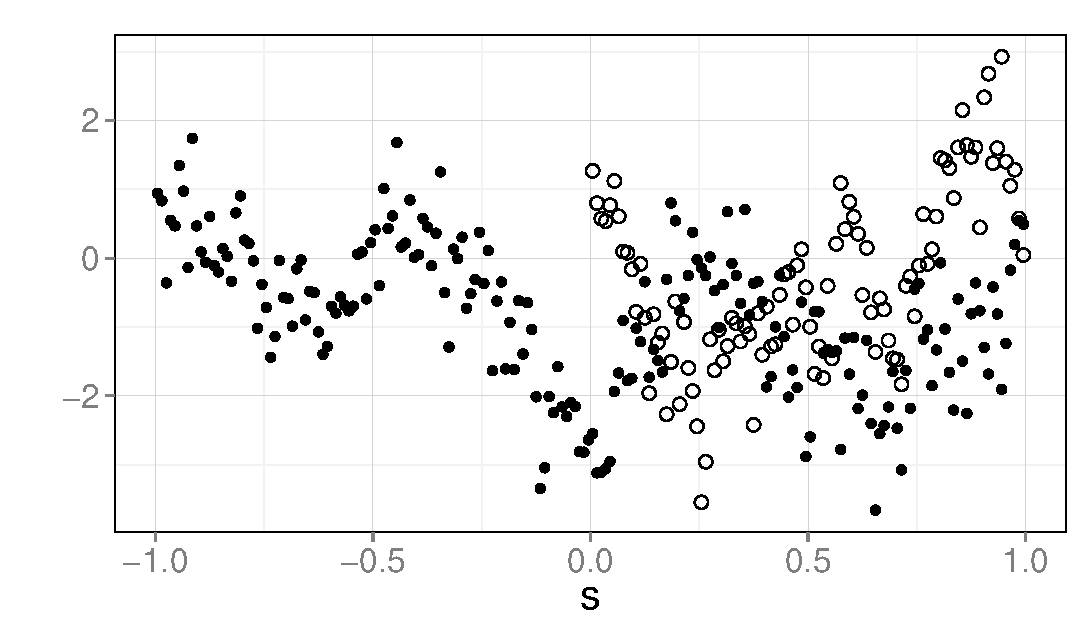
\includegraphics[width=2.7in]{../Conditional-approach-code/sim_obs.eps} \\
% & \hspace{-0.3in}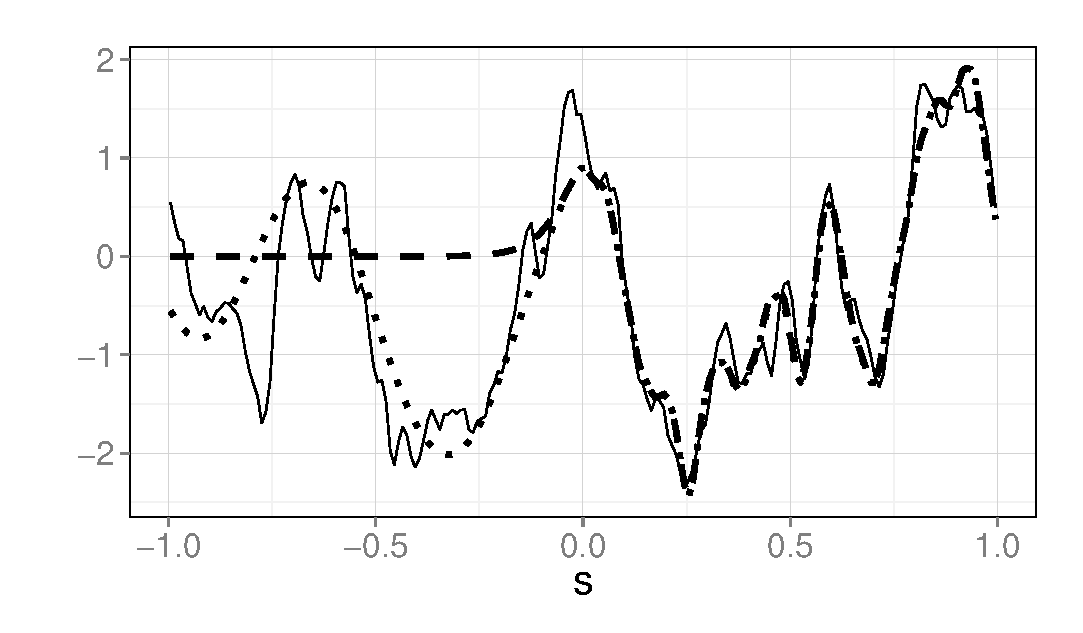
\includegraphics[width=2.9in]{../Conditional-approach-code/sim_est.eps} 
% \multirow{-2}[30]{*}{\figurebox{20pc}{}{}[Sigma.eps]} & \hspace{-0.5in} \figurebox{20pc}{}{}[sim_obs.eps] \\
%& 
\figurebox{15pc}{}{}[Fig1.eps] 
%\end{tabular}
%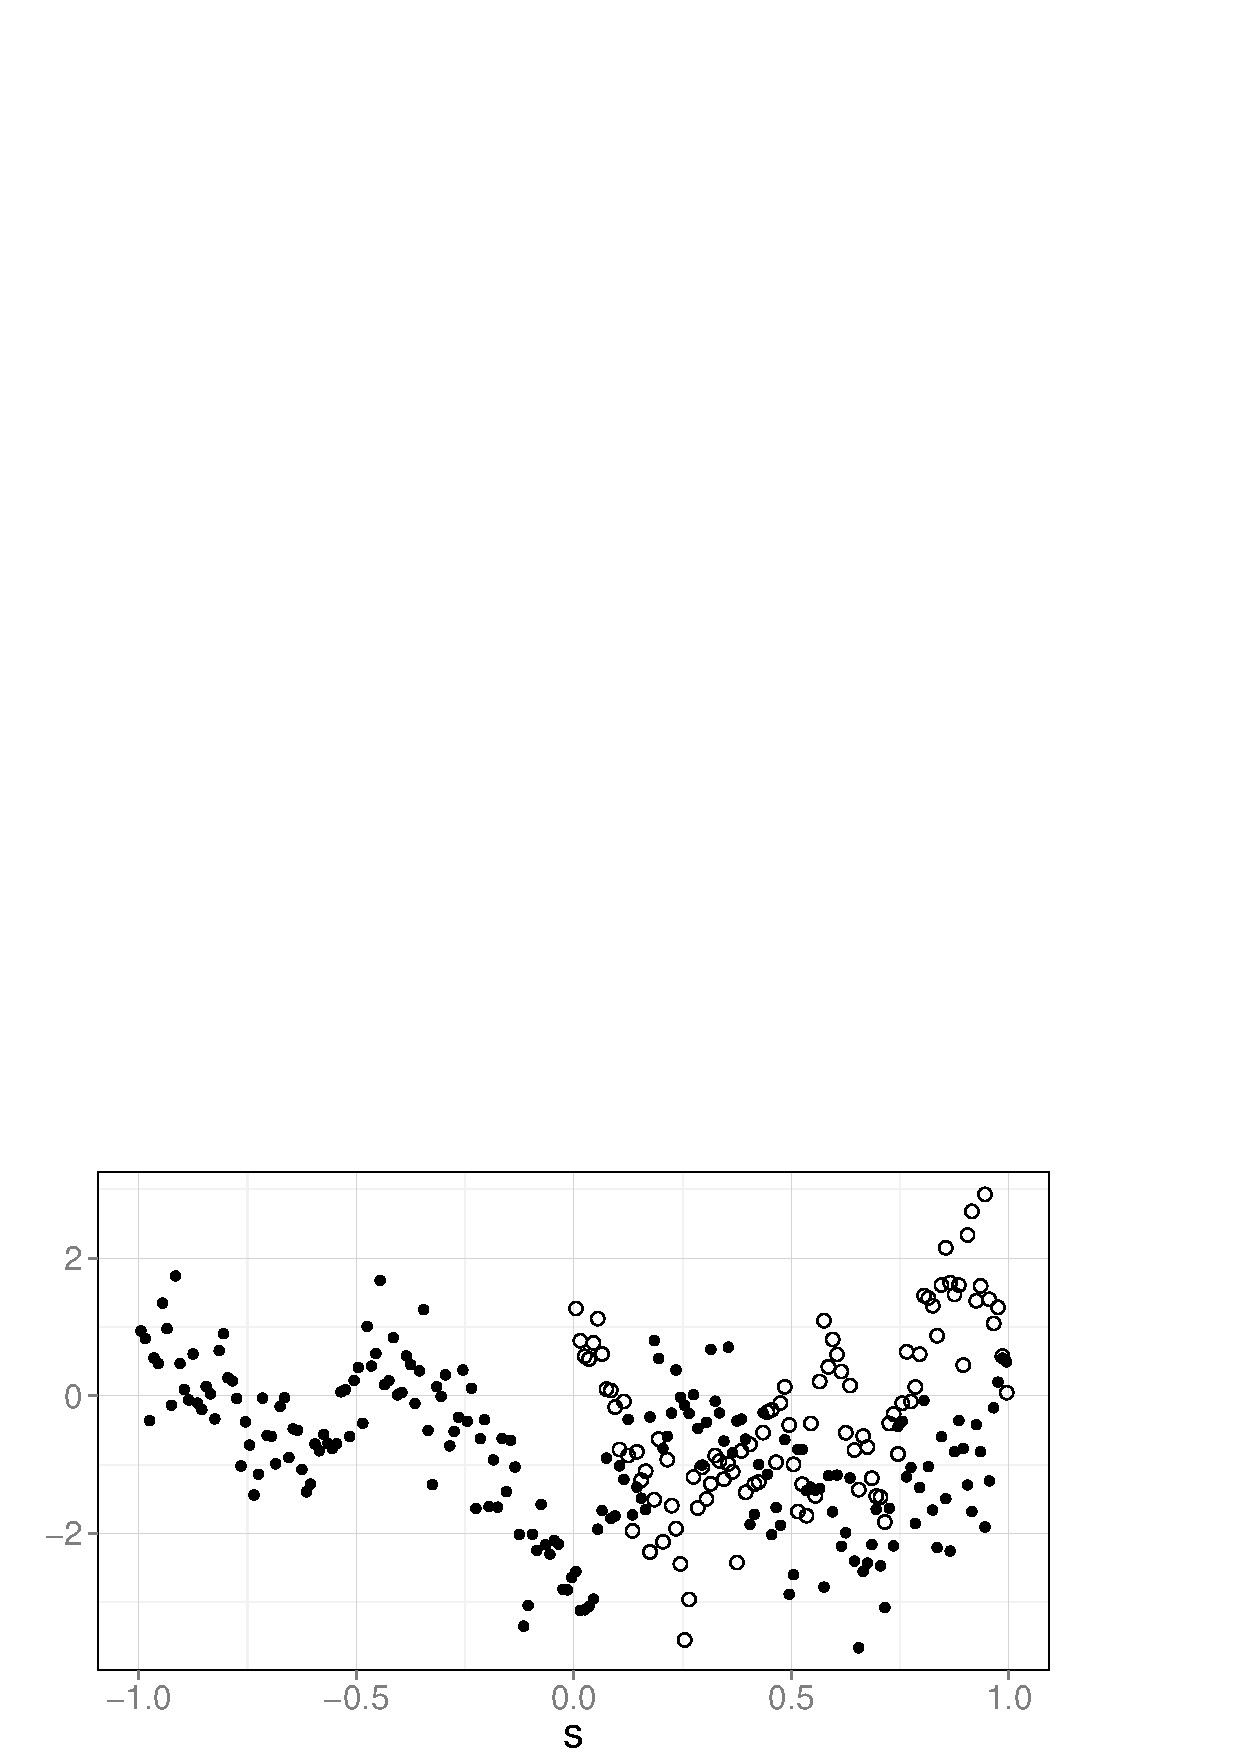
\includegraphics[width=3in]{../Conditional-approach-code/sim_obs.png}
%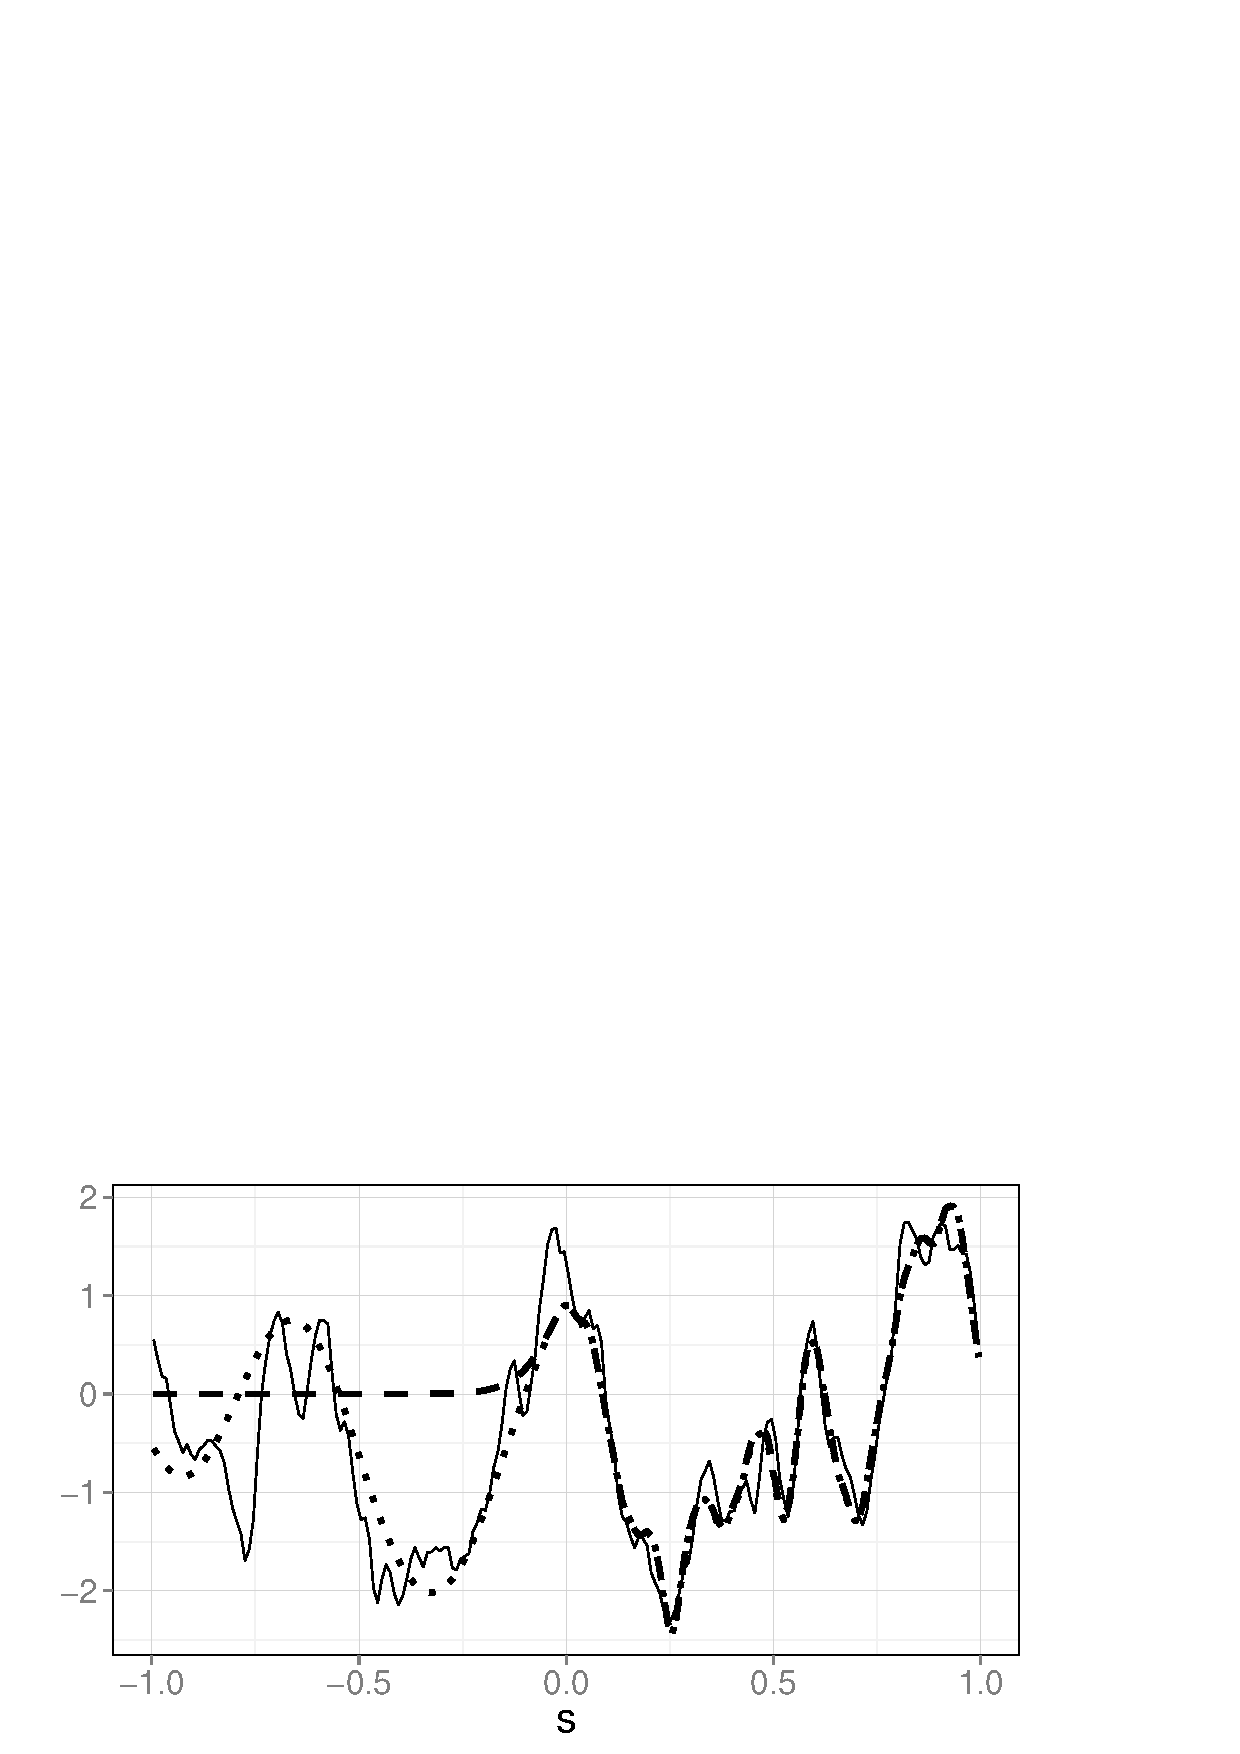
\includegraphics[width=3in]{../Conditional-approach-code/sim_est.png}
	\caption{Cokriging using spatial covariances defined by the conditional approach. Left panel: The covariance matrix \eqref{eqn:cov-matrix}. Right panel, top: The simulated observations $\Zvec_1$ (open circles) and $\Zvec_2$ (dots). Right panel, bottom: The hidden value $\Yvec_1$ (solid line), the kriging predictor $\widetilde\Yvec_1$ (dashed line), and the cokriging predictor $\hat\Yvec_1$ (dotted line).} \label{fig:sim}
%\end{center}
\end{figure}

\subsection{Deriving classes of cross-covariance functions from marginal covariance functions}\label{sec:cross-cov}

The conditional approach may also be used to complement the joint approach. In particular, \citet{GentonKleiber2015} posed an open problem that seemed difficult when using the joint approach to modelling covariance functions; ``[G]iven two marginal covariances, what is the valid class of possible cross-covariances that still result in a nonnegative-definite covariances structure?''. A straightforward answer to this question is available through \eqref{eqn:cov1}: The class of cross-covariance functions is given by \eqref{eqn:cov2} for any integrable function $b(\svec,\v)$ such that the function $C_{2\mid 1}(\cdot,\cdot)$ obtained from \eqref{eqn:cov1} is nonnegative-definite. This is potentially a very rich class of cross-covariance functions, and answering the question reduces to verifying which choice of $b(\cdot,\cdot)$ in \eqref{eqn:cov1} yields a nonnegative-definite $C_{2|1}(\cdot,\cdot)$.

For example, consider the stationary case in $D = \mathbb{R}^2$ where we have stationary covariance functions $C_{11}(\h), C_{2\mid 1}(\h)$, and interaction function $b(\s,\v) = b_o(\v - \svec)$ and let $D = \RR^2$. Then from \eqref{eqn:cov1},
\begin{equation*}
C_{2\mid 1}(\h) = C_{22}(\h) - \int_{\mathbb{R}^2}\int_{\mathbb{R}^2}{b_o(\tilde\v)b_o(\tilde\w)C_{11}(\h - \tilde\v + \tilde\w)\,\d\tilde\v\d\tilde\w}.
\end{equation*}
\noindent Let $\omegab \in \mathbb{R}^2$ denote spatial frequency, and let $\Gamma_{11}(\omegab), \Gamma_{22}(\omegab)$ and $B_o(\omegab)$ be the Fourier transforms of $C_{11}(\h), C_{22}(\h)$, and $b_o(\h)$, respectively. Then, for $C_{2\mid 1}(\h)$ to be a valid covariance function, it is required that $\Gamma_{22}(\omegab) - B_o(\omegab)B_o(-\omegab)\Gamma_{11}(\omegab)$ be nonnegative and integrable over $\omegab \in \mathbb{R}^2$ \citep{Cressie_1999,Gneiting_2002}. The inequality is trivial if $\Gamma_{11}(\omegab) = 0$; hence consider those $\omegab \in \Omega$ for which 
\begin{equation}\label{eq:B_ineq}
B_o(\omegab)B_o(-\omegab) \le \Gamma_{22}(\omegab)/\Gamma_{11}(\omegab),
\end{equation}
where $\Gamma_{11}(\omegab) > 0$. Recall that $C_{11}(\h)$ and $C_{22}(\h)$ are covariance functions and hence, necessarily, $\Gamma_{11}(\omegab) \ge 0$ and $\Gamma_{22}(\omegab) \ge 0$.

Any $B_o(\cdot)$ that satisfies \eqref{eq:B_ineq} gives the required result, since then finiteness follows from $\int\Gamma_{22}(\omegab)\,\intd\omegab < \infty$ being an upperbound on the integral, $\int \Gamma_{22}(\omegab) - B_o(\omegab)B_o(-\omegab)\Gamma_{11}(\omegab)\,\intd\omegab$. In Appendix 1, we show how a class of valid Mat{\'e}rn cross-covariance functions developed by \citet{Gneitingetal2010} can be obtained from \eqref{eq:B_ineq}.


\section{Multivariate spatial models through conditioning}\label{sec:4}

\subsection{Cross-covariance function definition}

In this section, we extend the conditional approach to the multivariate case. Initially, we work with the variables in their original ordering and subsequently show how graphical models define the general case. Now, $[Y_1(\cdot),\dots,Y_p(\cdot)]$ can be decomposed as, 

\begin{equation}\label{eq:decomp}
[Y_p(\cdot) \mid  Y_{p-1}(\cdot),Y_{p-2}(\cdot),\dots,Y_1(\cdot)][Y_{p-1}(\cdot) \mid  Y_{p-2}(\cdot),\dots,Y_1(\cdot)]\dots [Y_1(\cdot)].
\end{equation}
Analogous to the bivariate case $p=2$, we define the first two conditional moments of $Y_q(\cdot)$, for $q = 1,\dots,p$, as
\begin{align}
\E(Y_q(\svec) \mid  \{Y_r(\cdot) : r = 1,\dots,(q-1)\}) &= \sum_{r = 1}^{q-1} \int_D b_{qr}(\svec,\v)Y_r(\v) \intd \v; \quad \svec \in D, \label{eq:E_multi}\\
\cov(Y_q(\svec), Y_q(\uvec) \mid  \{Y_r(\cdot) : r = 1,\dots,(q-1)\}) &= C_{q \mid  r < q}(\svec,\uvec); \quad \svec,\uvec \in \mathbb{R}^d, \label{eq:cov_multi}
\end{align}
where $\{b_{qr}(\cdot,\cdot) : r = 1,\dots,(q-1) ;~q = 2,\dots,p\}$ are integrable functions that describe the conditional relationship of the $r$th process on the $q$th process.

As a result of the decomposition in \eqref{eq:decomp}, we obtain from \eqref{eq:E_multi} and \eqref{eq:cov_multi} the following expression for the marginal covariance function:
\begin{align}
C_{qq}(\svec,\uvec) &\equiv \cov(Y_q(\svec), Y_q(\uvec)) \nonumber \\
 & = C_{q \mid  (r<q)}(\svec,\uvec) + \sum_{r=1}^{q-1} \sum_{r'=1}^{q-1} \int_D\int_D b_{qr}(\svec,\v)C_{rr'}(\v,\w)b_{qr'}(\uvec,\w)\intd\v\intd\w, \label{eq:Cqq}
\end{align}
\noindent and for $r=1,\dots,q-1$ cross-covariance functions,
\begin{align}
C_{rq}(\svec,\uvec) &\equiv \cov(Y_r(\svec), Y_q(\uvec)) = \sum_{r'=1}^{q-1} \int_D\int_D b_{qr'}(\uvec,\w)C_{rr'}(\svec,\w)\intd\w. \label{eq:Crq}
\end{align}
Expressions \eqref{eq:Cqq} and \eqref{eq:Crq} are valid for $q=2,\dots,p$, and hence all covariance functions $\{C_{qr}:q,r=1,\dots,p\}$ are defined by $C_{qr}(\svec,\uvec) = C_{rq}(\uvec,\svec);~\svec,\uvec \in D$.

\subsection{Existence of a multivariate process}\label{sec:exist2}

Let $\{(Y_1(\svec),\dots,Y_p(\svec)): \svec \in \mathbb{R}^d\}, p \ge 2$ be a multivariate Gaussian process with mean $\bzero$. Following the discussion in Section \ref{sec:3-1}, the existence of the $p$-variate Gaussian process relies on the condition 
\begin{equation}\label{eq:Jp}
J_p \equiv \var\left(\sum_{q=1}^p \sum_{m=1}^{n_q} a_{qm}Y_q(\svec_{qk})\right) \ge 0,
\end{equation}
for any real numbers $\{a_{qm}: m = 1,\dots,n_q; q = 1,\dots,p\}$, any nonnegative integers $\{n_q: q=1,\dots,p\}$ such that $n_1 + \dots + n_p > 0$, and any $\{\svec_{qk} : k = 1,\dots,n_q;~q = 1,\dots, p\}$. The proof showing that \eqref{eq:Jp} is satisfied under these conditions follows by induction. We have already shown, through \eqref{eqn:left-hand-of-var}, that $J_2 \ge 0$. Assume that $J_{p-1} \ge 0$. Then, it can be shown by using the identities in \eqref{eq:Cqq} and \eqref{eq:Crq} that  \eqref{eq:Jp} is given by
\begin{equation*}
  J_p= \sum_{m=1}^{n_p}\sum_{m'=1}^{n_p}a_{pm}a_{pm'}C_{p \mid  (q < p)}(\svec_{pm},\svec_{pm'}) + \int_D\int_Da_q(\svec)a_r(\uvec)C_{qr}(\svec,\uvec)\intd \svec \intd \uvec,
\end{equation*}
\noindent where 
\begin{equation}\label{eq:a_def2}
a_q(\svec) \equiv \left(\sum_{k=1}^{n_q}a_{qk}\delta(\svec - \svec_{qk}) + \sum_{m=1}^{n_p}a_{pm}b_{pq}(\svec_{pm},\svec)\right).
\end{equation}
Hence, \eqref{eq:Jp} holds for all $p \ge 2$. For a full derivation see Appendix 2.

This result implies that a multivariate spatial Gaussian model constructed using the conditional approach \eqref{eq:E_multi} and \eqref{eq:cov_multi} exists, provided that univariate $C_{11}(\cdot,\cdot)$ and $\{C_{q \mid  (r < q)}(\cdot,\cdot): q = 1,\dots,p\}$ are valid covariance functions, and interaction functions $\{b_{qr}(\cdot,\cdot) : r = 1,\dots,q-1;~q = 2,\dots,p\}$ are integrable. 

\subsection{A graphical model representation}

Because any joint model can be decomposed using \eqref{eq:decomp}, the existence result in Section \ref{sec:exist2} holds for systems that do not exhibit any particular structure, and recall that the marginal processes themselves need not be isotropic nor stationary. Here, we give examples of implementation of the conditional approach, such as can be found in non-spatial settings \citep[e.g.,~][]{Cox_1996}.

Consider the trivariate case of $p=3$; clearly the decomposition \eqref{eq:decomp} is not unique: The joint probability measure can be written as
\begin{equation*}
[Y_1(\cdot),Y_2(\cdot),Y_3(\cdot)]=[Y_3(\cdot)\mid Y_1(\cdot),Y_2(\cdot)][Y_2(\cdot)\mid Y_1(\cdot)][Y_1(\cdot)],
\end{equation*}
and equally,
\begin{equation*}
[Y_1(\cdot),Y_2(\cdot),Y_3(\cdot)]=[Y_1(\cdot)\mid Y_2(\cdot),Y_3(\cdot)][Y_2(\cdot)\mid Y_3(\cdot)][Y_3(\cdot)].
\end{equation*}
Indeed there are a total of six such possible models (in the bivariate case, there are two possible models). 

When building classes of models, it is generally better to have more choice, but in the conditional approach we can be guided by a graph structure. For example, in the bivariate case considered by \citet{Royleetal1999}, node 1 is defined by the pressure field $Y_1(\cdot)$ and node 2 is defined by the wind field $Y_2(\cdot)$. The direction of the edge in the directed graph is clearly from node 1 to node 2 and not the other way around, since wind fields are the result of differential pressures in the atmosphere. 

As in network analysis \citep[e.g.,][]{Kolaczyk_2009}, specification of the graph structure for spatial processes will be guided by a desire for parsimonious models. One example of a parsimonious conditionally-specified model  is the spatial moving average model of \cite{verHoef_1998}, where $p=5$. \cite{verHoef_1998} construct a bivariate model $(Y_1(\cdot),Y_2(\cdot))$ by taking moving averages of a combination of correlated processes $(Y_3(\cdot),Y_4(\cdot),Y_5(\cdot))$, where the following decomposition is implicitly assumed, 
\begin{align}\label{eq:verHoef}
[Y_1(\cdot),\dots,Y_5(\cdot)] &= [Y_1(\cdot) \mid  Y_3(\cdot)][Y_2(\cdot)\mid Y_4(\cdot)][Y_3(\cdot)\mid Y_5(\cdot)][Y_4(\cdot)\mid Y_5(\cdot)][Y_5(\cdot)].
\end{align}
\noindent In \eqref{eq:verHoef}, $[Y_1(\cdot) \mid  Y_3(\cdot)]$ and $[Y_2(\cdot) \mid  Y_4(\cdot)]$ are constructed using moving average functions of the form $b(\s,\v) = b_o(\v - \s)$ in \eqref{eqn:E-and-cov}; $[Y_3(\cdot)\mid Y_5(\cdot)]$ and $[Y_4(\cdot)\mid Y_5(\cdot)]$ assume Dirac-delta functions; and $Y_5(\cdot)$ is a white-noise process. 

An important special case is commonly seen in studies of spatio-temporal phenomena. In such settings, each process is indexed by time $t=1,\cdots,p$, and nodes $1,\dots,p$ are connected successively by directed edges. This results in the Markov factorization:
\begin{equation}\label{eq:Markov}
[Y_1(\cdot),\dots,Y_p(\cdot)]=[Y_1(\cdot)]\prod_{t=2}^p[Y_t(\cdot)\mid Y_{t-1}(\cdot)].
\end{equation}
%\noindent \red{\texttt{***Andrew to make clearer***}}. In this case, a further parsimonious simplification for large $p$ could be the constraint that $\cov(Y_q(\s),Y_{q+l}(\s + \h))$, for some integer $l$, is independent of both $\h$ \emph{and} $q$. This is easily achieved in the conditional approach by letting $b(\cdot,\cdot)$ be a convolution kernel and $C_{q\mid q-1}(\h)$ be independent of $q$ \citep{Storvik_2002}.


%Even if the directions are known, in practice, as we shall see next, both the graphical structures and the functions which need to pre-specified are usually constrained to aid inference.

\subsection{The conditional approach provides spatial model flexibility}

It is easy to see that the number of covariance and interaction functions that need to be specified is $p(p+1)/2$, which is also the number of elements in the lower triangle of a $p \times p$ cross-covariance function matrix. Hence, the modeller using the conditional approach provides up to $p(p+1)/2$ univariate nonnegative-definite and integrable functions in order to specify the $p(p+1)/2$ marginal and cross-covariance functions. Critically, specification of any one function does not constrain specification of the others. This flexbility is not necessarily present in other commonly used approaches to multivariate spatial model construction. For example, both in the convolution method of \citet{MajumdarGelfand2007}, and in the linear model of coregionalization, the user is allowed a choice of at most $p$ covariance functions. 




\section{Bivariate spatial modelling of temperature data using the conditional approach}\label{sec:5}

\subsection{The data}

We demonstrate the flexibility of the conditional approach on the bivariate minimum/maximum temperature dataset used in \cite{GentonKleiber2015}. The data are minimum-temperature and maximum-temperature residuals in the state of Colorado, USA (following the removal of the state-wide mean) obtained from measurements taken on September 19, 2004 at 94 weather stations in Colorado; that is, $m_1 = m_2 = m = 94$ and $D_1^O = D_2^O = D^O$. Minimum temperatures are likely to have occurred in the early morning hours of a given day, with the maximum temperatures in the afternoon of the same day. It is natural then to assume that the maximum-temperature residual later in the day is partially determined by the minimum-temperature residual in the early morning. Consequently, time induces a bivariate dependence that can be modelled naturally using a conditional approach.  %The conditional approach lends itself nicely to such applications where the causal direction is readily apparent.

%The scope of this section is twofold; first, to exemplify the rich class of models which can be applied using this single framework and, second, to demonstrate how computational methods can be used to integrate the conditional approach within a fully Bayesian framework, including Bayesian model comparison, for use within a practical setting.

\subsection{The model}

In this subsection, we propose a Bayesian hierarchical model with spatial dependence in the process model and  prior distributions on the unknown parameters. Let $Y_1(\cdot)$ and $Y_2(\cdot)$ denote the true minimum-temperature and maximum-temperature residuals, respectively. Let $\epsilonb(\cdot) \equiv (\varepsilon_1(\cdot),\varepsilon_2(\cdot))^\T$ be the bivariate process of measurement errors or potential measurement errors, and assume that the data or potential data, $\Zvec(\cdot) \equiv (Z_1(\cdot),Z_2(\cdot))^\T$ are related to $\Yvec(\cdot) \equiv (Y_1(\cdot),Y_2(\cdot))^\T$ through, $\Zvec(\cdot) = \Yvec(\cdot) + \epsilonb(\cdot)$. The two measurement errors are assumed to have no spatial dependence, but they could be correlated, which we model through
\begin{equation*}
\cov(\epsilonb(\svec)) = \sigma^2_\varepsilon \begin{bmatrix} 1 & \rho_\varepsilon \\ \rho_\varepsilon & 1 \end{bmatrix}; \quad \textrm{for}~ \rho_\varepsilon \in (-1,1) ~ \textrm{and} ~ \svec \in D.
\end{equation*}

In the conditional approach, we need to specify the univariate covariance functions, $C_{11}(\svec,\uvec)$ and $C_{2\mid 1}(\svec,\uvec)$, and the integrable interaction function $b(\svec,\v)$. We let the covariance functions be isotropic Mat{\'e}rn covariance functions given by \eqref{eq:Matern1} and \eqref{eq:Matern2}. The smoothness parameters $\nu_{11}$ and $\nu_{2\mid 1}$ are set equal to 1.5, to give a covariance function that is a little smoother than the exponential covariance function. We let $b(\svec,\v)$ be a function of displacement, $\h \equiv \v - \svec$, and recall that $b_o(\h) \equiv b(\svec,\v)$. Write the three different models that we fit as:
\begin{equation*}
\begin{array}{ll}
\textrm{Model 1 (independence):} &b_o(\h) \equiv 0, \\
\textrm{Model 2 (pointwise dependence):} &b_o(\h) \equiv A\delta(\h), \\
\textrm{Model 3 (diffused dependence):} &b_o(\h) \equiv \left\{\begin{array}{ll} A\{1 - (\|\h - \Deltab\|/r)^2\}^2, & \| \h - \Deltab\| \le r \\ 0, & \textrm{otherwise}, \end{array} \right. 
\end{array}
\end{equation*}

\noindent where $\Deltab = (\Delta_1, \Delta_2)^\T$ is a shift parameter that captures asymmetry. In Model 3, $b_o(\h)$ is a shifted bisquare function in $\mathbb{R}^2$, which is analogous to \eqref{eq:bisquare1D} given in $\mathbb{R}^1$.

We discretized both $Y_1(\cdot)$ and $Y_2(\cdot)$ using a triangulated grid with $n_1= n_2 = n = 968$ vertices each. Here, the vertices of the grid define $D^L$, an irregular spatial lattice; see Fig.~\ref{fig:mesh}.
%In this work, to maintain a consistent inference framework across all models, we decompose $Y_1(\cdot)$ and  using a triangulated mesh and apply the stochastic partial differential approach \citep[SPDE][]{Lindgren_2011} in order to obtain a sparse approximation of $\left(\{C_{11}(\svec_i,\svec_j)\}_{i,j=1}^{n_1}\right)^{-1}$. Since $n_1$, the number of vertices, needs to be large to obtain an accurate approximation to $Y_2(\svec) \mid  Y_1(\cdot)$ (we use $n_1 = 2147$), the sparse representation becomes useful for quick sampling in a Markov chain Monte Carlo (MCMC) setup. In contrast, an accurate decomposition of $Y_2(\cdot)$ is not essential for parameter inference and we can work directly with the covariance matrix $\{C_{2\mid 1}(\svec_i,\svec_j)\}_{i,j=1}^{n_2}$ in its dense form, considering only $Y_2(\svec_i)$ for each observation location $\svec_i$ (hence $n_2 = 94$). We denote $Y_1(\cdot)$ evaluated at the mesh locations as $\Yvec_1 \in \mathbb{R}^{n_1}$ and $Y_2(\cdot)$ evaluated at the observation locations as $\Yvec_2 \in \mathbb{R}^{n_2}$, see Fig.~\ref{fig:mesh_kernel}, left. Since the SPDE approach in two-dimensions can only be used for integer values of $\nu$ we fix $\nu_{11} = 2$, whilst for fast computation of the elements of $\{C_{2\mid 1}(\svec_i,\svec_j)\}_{i,j=1}^{n_2}$ we fix $\nu_{2\mid 1} = 1.5$.
Under the chosen triangulation, the integral in \eqref{eqn:E-and-cov} is approximated as $\E(Y_2(\svec_l) \mid  Y_1(\cdot)) \simeq \sum_{k=1}^{n} \eta_k b(\svec_l,\v_k)Y_1(\v_k)$, where in this case $\{\eta_k: l = 1,\dots,n\}$ are the areas of the Voronoi tessellations constructed from the triangulated grid \citep[e.g.,][]{Lee_1980}.

 \begin{figure}[!t]
% 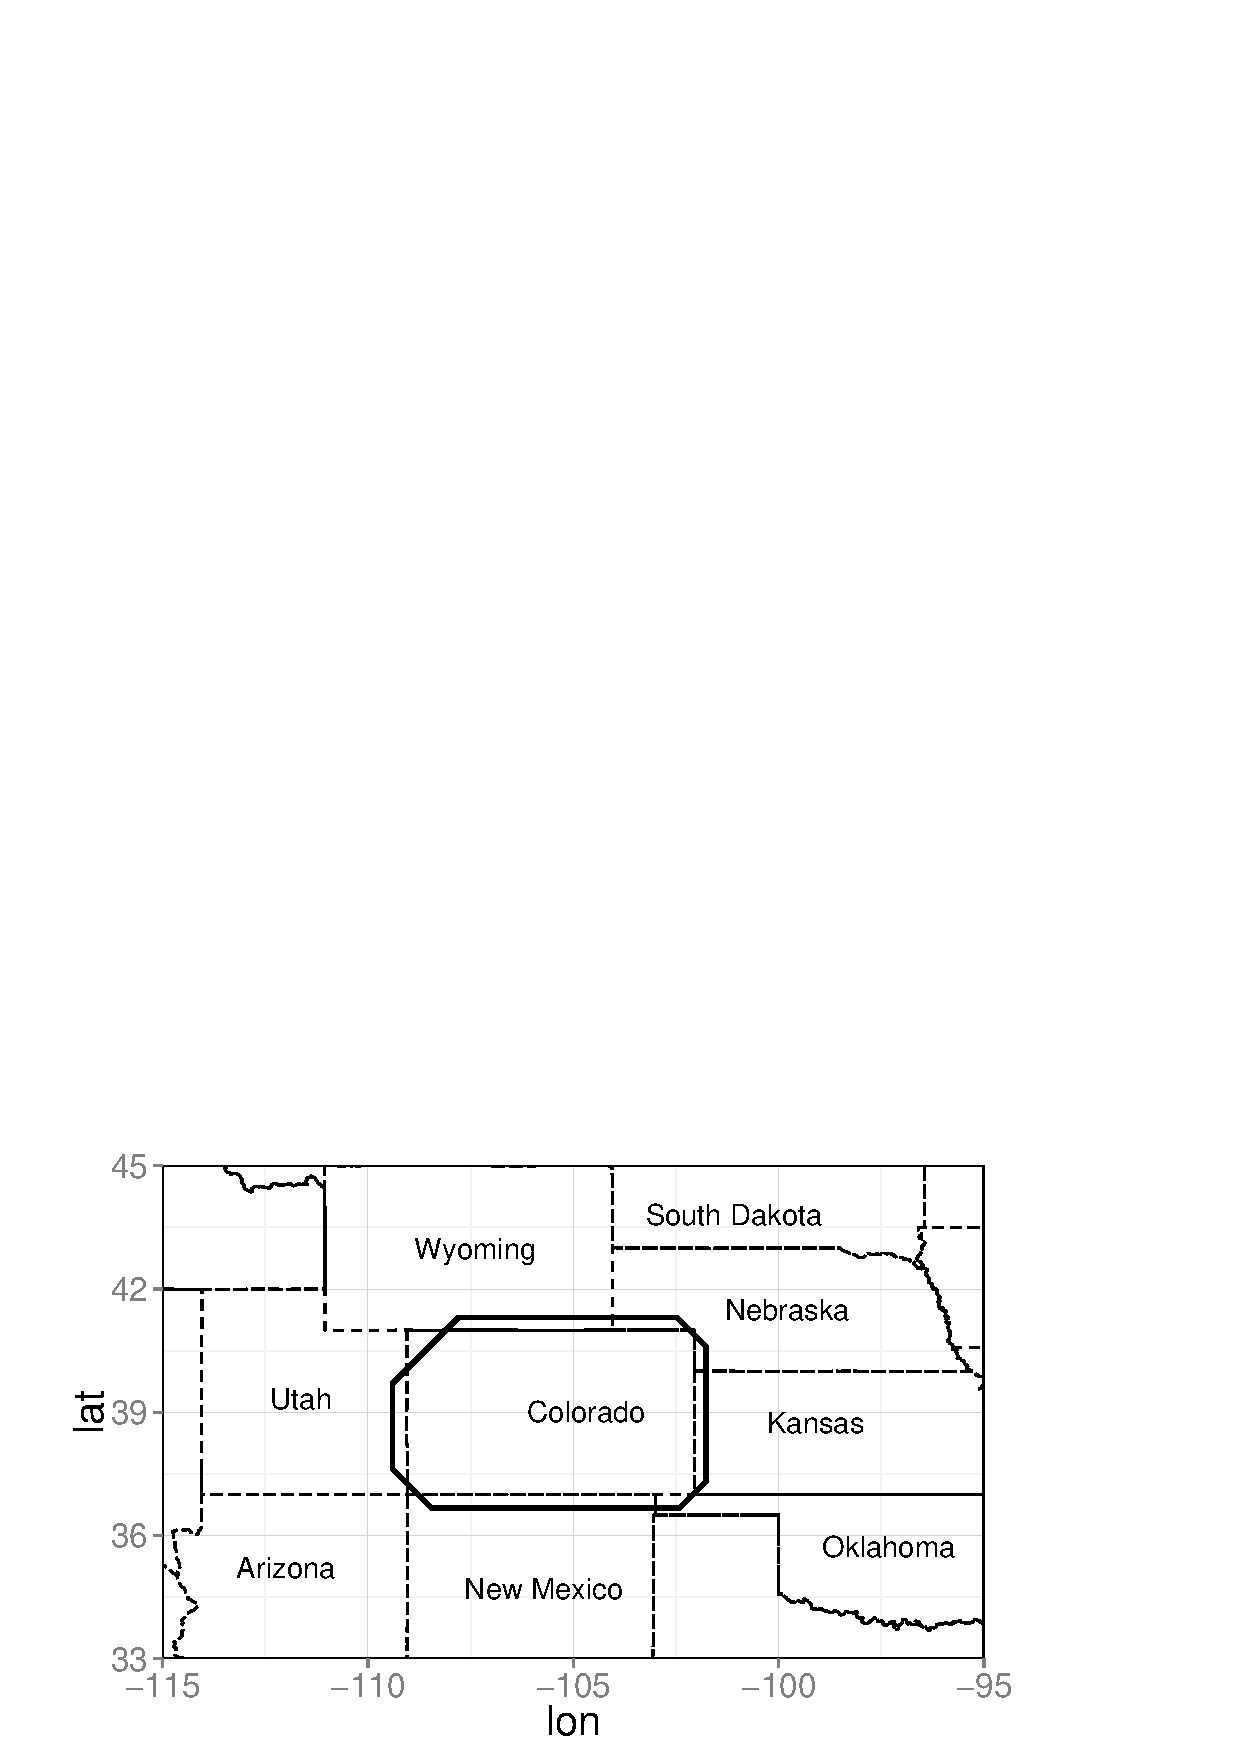
\includegraphics[width=2.8in]{../Conditional-approach-code/Stateplot.png}
\figurebox{10pc}{}{}[Fig2.eps]
% 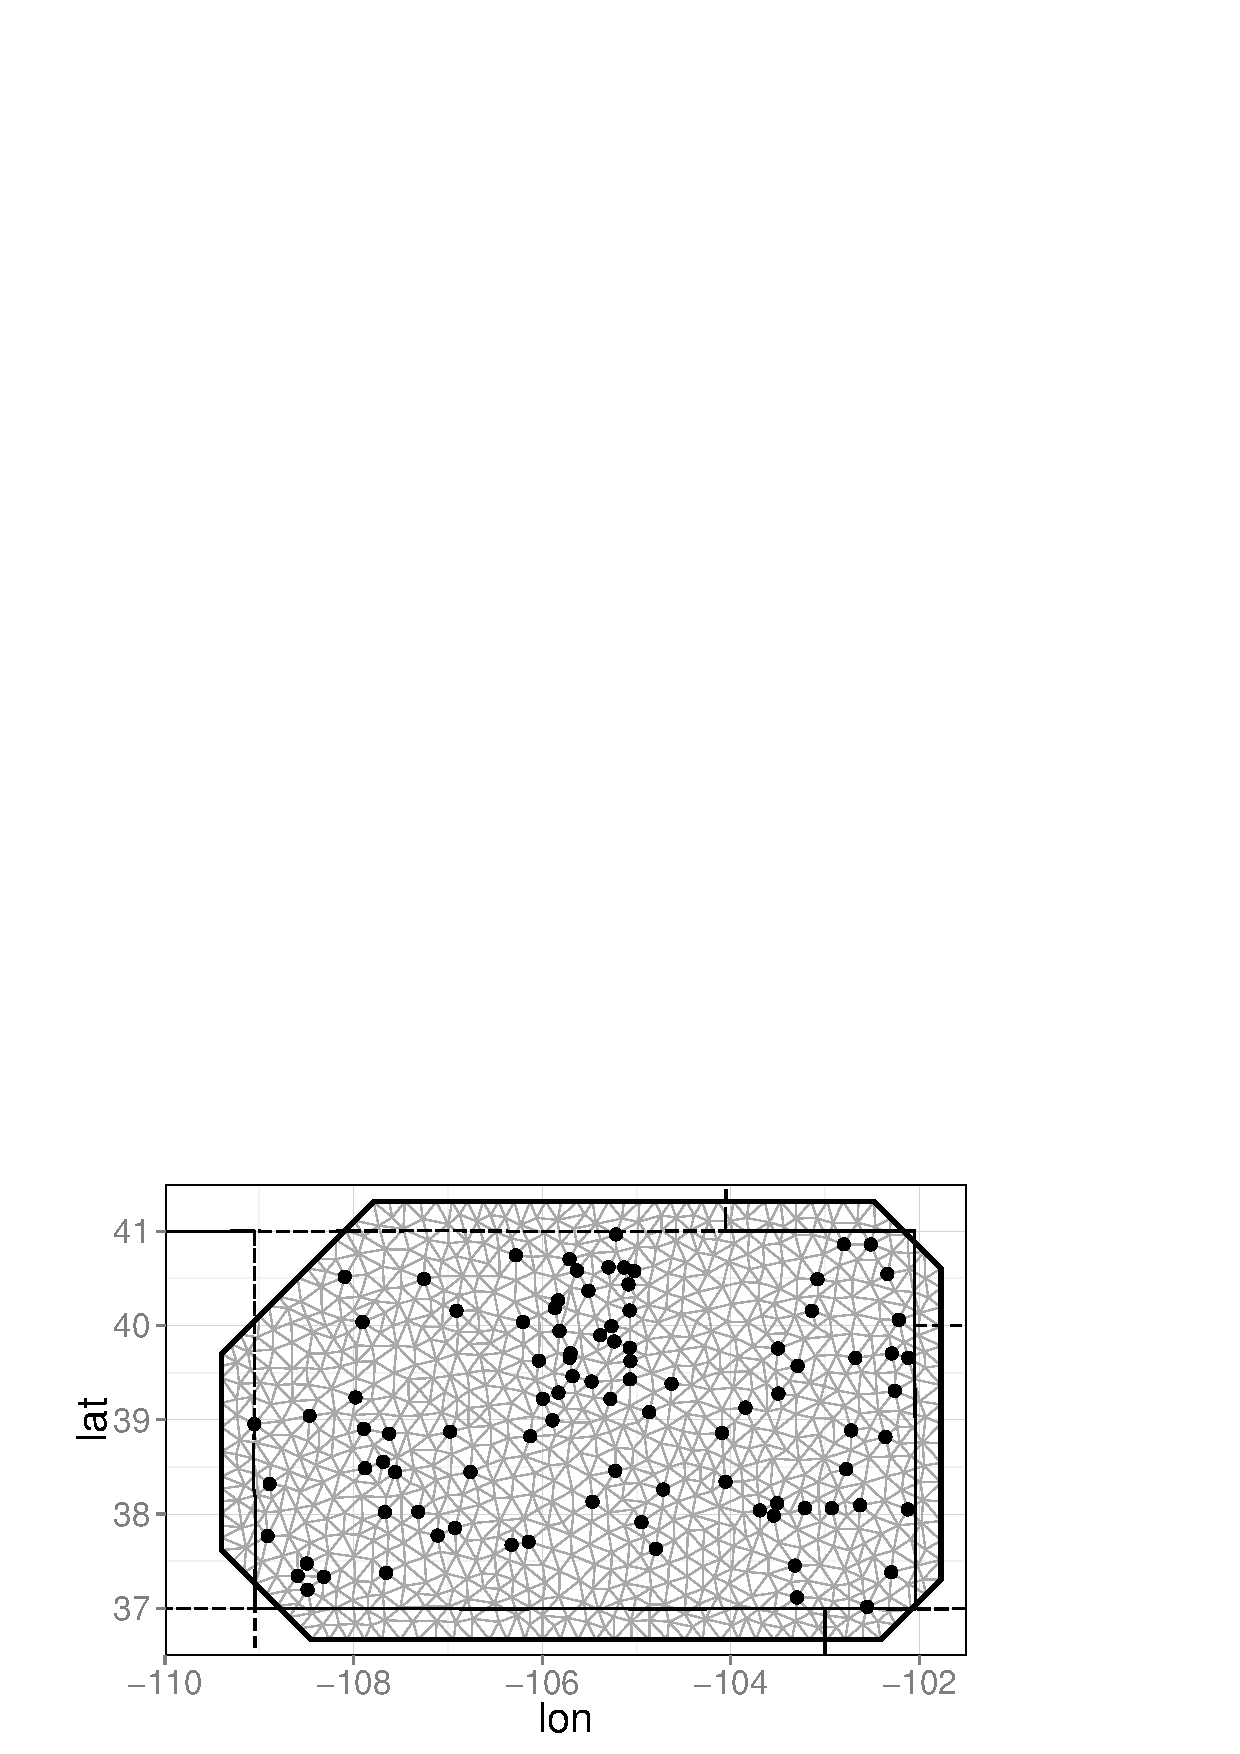
\includegraphics[width=2.8in]{../Conditional-approach-code/meshplot.png}
 	\caption{Left panel: State boundaries in a region of the USA (dashed lines), with the domain of interest enclosed by a bounding polygon (solid line). Right panel: The irregular triangular grid used for discretising $D$. The observation locations given by $D^O$ consist of the large dots and the discretized spatial domain $D^L$ consists of the mesh nodes.} \label{fig:mesh}
 \end{figure}

 \begin{figure}[!t]
% \begin{center}
% \begin{tabular}{cc}
% \includegraphics[width=2.8in]{../Conditional-approach-code/Y1est.png} & \multirow{-2}[30]{*}{\includegraphics[width=3in]{../Conditional-approach-code/Denver_FortCollins_vector.png}} \\
% \includegraphics[width=2.8in]{../Conditional-approach-code/Y2est.png} 
% \end{tabular}
\figurebox{19pc}{}{}[Fig3.eps]
 	\caption{Results for Model 3. Left panel: Interpolated maps in degrees Celsius (degC) of $\E(\Yvec_1 \mid  \Zvec_1,\Zvec_2)$ and $\E(\Yvec_2 \mid  \Zvec_1, \Zvec_2)$. Right panel: Prior (light grey) and posterior (dark grey) median (solid line) and inter-quartile ranges (enclosed by dashed lines) of the interaction function $b_o(\cdot)$ of Model 3, along a unit vector $\e$ originating at Denver (DE) in the direction of Fort Collins (FC).} \label{fig:kernel}
% \end{center}
 \end{figure}

\red{***Check***} We employ a Bayesian hierarchical model and place prior distributions on transformations of the parameters, with each transformation chosen to account for the range of its respective parameter. The prior distributions and transformations are summarized in Table \ref{tab:priors} (given in Appendix 3). Elicited prior distributions reflect some prior understanding of the problem: For example, we can reasonably expect that the error $\sigma_\varepsilon$ will lie between 0.5 and 2 degrees Celsius, and thus we place a Gamma prior on $\sigma_\varepsilon^{-2}$ such that $q_{0.05}(\sigma_\varepsilon) =0.05$ and $q_{0.95}(\sigma_\varepsilon) = 2$, where $q_x(\cdot)$ denotes the $x$th quantile of its argument.

%In particular, since
%\begin{itemize}
%\item $\rho_\varepsilon$ is bound by (-1,1), we define $\rho_\varepsilon \equiv 2\Phi(\gamma_{\rho_\varepsilon}) - 1$ and place a Gaussian prior on $\gamma_{\rho_\varepsilon}$.
%\item $\kappa_{11}$ and $\kappa_{2\mid 1}$ are strictly positive, we define  $\kappa_{11} \equiv \exp(\gamma_{\kappa_1})$ and $\kappa_{2\mid 1} \equiv \exp(\gamma_{\kappa_{2\mid 1}})$ and place Gaussian priors on $\gamma_{\kappa_{11}}$ and $\gamma_{\kappa_{2\mid 1}}$.
%\item $r$ is positive, we define  $r \equiv \exp(\gamma_{r})$ and place a Gaussian prior on $\gamma_{r}$.
%\item we will be working largely with precision matrices, we consider the precisions $\sigma^{-2}_\varepsilon,\sigma^{-2}_{11},\sigma^{-2}_{2\mid 1}$ instead of the variances $\sigma^{2}_\varepsilon,\sigma^{2}_{11},\sigma^{2}_{2\mid 1}$ and place Gamma priors on each of these.
%\end{itemize}

%Since all fields are directly observed, the prior judgments need not be largely informative. However in this and similar case studies, reasonable choices for the hyperparameters should be made due to data paucity and the relatively large number of unknowns. All prior distributions shown in the summary of Table \ref{tab:priors} reflect such choices. For example, we can reasonably expect the error $\sigma_\varepsilon$ to be lie roughly between 0.5 and 2 degrees and have thus placed a Gamma prior on $\sigma_\varepsilon^{-2}$ such that $q_{0.05}(\sigma_\varepsilon) =0.05$ and $q_{0.95}(\sigma_\varepsilon) = 2$, where $q_x(\cdot)$ denotes the $x^{th}$ quantile of its argument.




%The computational approach taken depends to a large extent on the treatment of $\Yvec(\svec)$ and this, in turn, depends on the intended scope of the analysis. At the very least, for Models 1 and 2, one should consider $\Yvec(\svec)$ at each of the observation locations. For Model 3, since $Y_2(\cdot)$ depends on the \emph{whole} of $Y_1(\cdot)$, at the very least one also needs to consider a suitable fine-scale discretisation of $Y_1(\cdot)$.


\subsection{Inference and model comparison}

For posterior inference we employed a Gibbs sampler. Through the use of conjugate priors, we obtained conditional distributions of standard form for $\sigma^2_\epsilon, \Yvec, A,\sigma^2_{11}$, and $\sigma^2_{2\mid 1}$ (see Table \ref{tab:priors}, Appendix 3), from which we were able to sample directly. Since the conditional distributions for the remaining parameters, namely $\rho_\varepsilon, \kappa_{11}, \kappa_{2\mid 1}, r, \Delta_1$, and $\Delta_2$, are nonstandard, we sampled from these using a slice sampler \citep{Neal_2003}. Slice samplers tend to be more efficient than simple Metropolis samplers, as they effectively alter the magnitude of the steps taken at each point in the chain by adapting to the local properties of the density function.  However, the computational effort for generating one sample is larger than for a standard Metropolis sampler.

We generated $N = 50,000$ samples from the slice-within-Gibbs Markov chain Monte Carlo scheme, discarded the first 1,000 for burn-in, and then thinned by only recording every 100th sample.  Slice sampling was carried out using the stepping-out method \citep[][Section 4]{Neal_2003} with an interval width adapted during the burn-in period. We used marginal samplers for $\rho_{\varepsilon},\kappa_{11}, \kappa_{2\mid 1}$, while for Model 3 we sampled $r,\Delta_1,$ and $\Delta_2$ jointly since these parameters can be expected to be highly correlated. For the slice samplers, we used the R \citep{R} package \texttt{slice} from the personal home page of Jonathan C. Rougier, University of Bristol. %\texttt{http://www.maths.bris.ac.uk/\~MAZJCR/}.

%In Method 3, the number of non-zeroes in $\Bmat$ changes throughout the MCMC scheme according to the sampled $r$. A large $r$ will decrease the number of non-zeroes and hence decrease the sparsity of the precision matrices. There comes a point where sparse linear algebraic techniques are in fact slower than dense matrix methods. We found that switching to dense matrix algebraic routines when the number of non-zeroes in $\Bmat$ exceeded 1\% considerably improved the average time required for a single sample.

 A summary of our parameter inferences are given in Table \ref{tab:results} (given in Appendix 3), while the posterior expectations of $Y_1(\svec)$ and $Y_2(\svec)$  are given in the left panel of Fig.~\ref{fig:kernel}. There the influence of the Rocky Mountains on the temperature residuals is apparent. In Fig.~\ref{fig:kernel}, right panel, we plot the interquartile ranges of the prior $[b_o(h\e)]$ and the posterior, $[b_o(h\e\mid \Zvec_1,\Zvec_2)]$, where $\e$ is the unit vector originating from Denver in the direction of Fort Collins. The posterior distribution of the interaction function along this direction can be clearly distinguished from the prior distribution, suggesting that Bayesian learning has uncovered substantial interaction between maximum temperature and minimum temperature at proximal locations. Model 3, for different choices of $b_o(\cdot)$, has in fact often been used to study the dynamics in spatio-temporal processes \citep{Kot_1986,Wikle_2002}.

%Such diffused dependence is commonly assumed when modelling spatial processes at different time points. It is thus no coincidence that the bivariate model with the chosen $b(\h)$ kernel is similar to several spatio-temporal models commonly employed in practice \citep[e.g.,][]{Kot_1986,Wikle_2002}.

%and $b(h\e)$ for Model 3 are given in Fig.~\ref{fig:kernel}.  is apparent in the left panels, and in the lower-right panel the kernel is relatively diffuse, indicating that the influence of $Y_1(\cdot)$  on $Y_2(\cdot)$ is not localised. There is a also a suggestion that the kernel is off-centre, and that the dependence could be influenced by some (unobserved) flow process. Model 3, for different choices of $b(\cdot)$, has in fact often been used to study the dynamics in spatio-temporal processes \citep{Kot_1986,Wikle_2002}.

%Although it is beyond the scope of this article to discuss the posterior summaries in detail, we note that $\rho_\varepsilon$ in all models is deemed to be negative while $\sigma^2_\varepsilon$ is larger than expected. This could be due to the lack of consideration of a fine-scale temperature residual process. Unfortunately, without knowledge of the error characteristics, the observation error and process fine-scale variation can not be resolved.

The Deviance Information Criterion \citep[DIC,][]{Spiegelhalter_2002} for the three models is given in the lower row of Table \ref{tab:results} in Appendix 3. The DIC penalizes a model for poor fit and model complexity; the lower the value, the more favourable the model. In our case, DIC is highest for Model 1 and lowest for Model 3, indicating that there are important bivariate interactions being captured by the latter. Interestingly, the DIC for Models 2 and 3 are comparable despite inferences on $\kappa_{2\mid 1}$ being very different for the two. One definition of the range parameter is the Euclidean distance, $\|\uvec - \svec\|$, where $C_{2\mid 1}(\svec,\uvec) = 0.1\sigma^2_{2\mid 1}$; \citet{Lindgren_2011} approximate it as $\lambda_{2\mid 1} \simeq (8\nu_{2\mid 1})^{1/2}/\E(\kappa_{2\mid 1} \mid  \Zvec_1, \Zvec_2)$. Model 2 essentially describes $Y_2(\cdot)$ as a scaled version of $Y_1(\cdot)$ with $\lambda_{2\mid 1} = 5.0$ degrees longitude/latitude. In contrast, Model 3 describes $Y_2(\cdot)$ as a diffused version of $Y_1(\cdot)$ with $\lambda_{2\mid 1} = 1.8$ degrees longitude/latitude. 

The models considered in this application range in complexity. The conditional approach allows for a quick analysis of various models with different spatial-dependence characteristics, solely by varying $b(\cdot,\cdot)$. It is easy to envision more complicated forms of $b(\cdot,\cdot)$, including ones motivated by causative scientific models of how $Y_2(\cdot)$ could depend on $Y_1(\cdot)$. 

% \subsection{Model comparison}

% The discrepancy between data and model can be be assessed using the \emph{deviance}
% \begin{equation}
% D(\Zvec,\Yvec,\thetab) \equiv -2 \log p(\Zvec\mid \Yvec,\thetab).
% \end{equation}
% \noindent Since the deviance is a function of the unknowns $\Yvec$ and $\thetab$ we use the average deviance from the posterior realisations of $(\Yvec, \thetab)$
% \begin{equation}
% \widehat D(\Zvec) \equiv \frac{1}{N}\sum_{i=1}^N D(\Zvec,\Yvec^{(i)},\thetab^{(i)}).
% \end{equation}

% The average deviance alone is not sufficient when comparing across models with differing complexities. In deviance-based strategies, a penalty for model complexity $p_D$ is obtained by computing the difference between $ \widehat D(\Zvec)$ and the deviance at the posterior means of $\Yvec,\thetab$, $D(\Zvec; \widehat \Yvec, \widehat \thetab)$. Then the \emph{Deviance Information Criterion} (DIC) is simply the addition of these two quantities \citep{Spiegelhalter_2002}:

% \begin{equation}
% DIC \equiv 2\widehat D(\Zvec) - D(\Zvec; \widehat\Yvec,\widehat\thetab).
% \end{equation}

% The mean deviance and the DIC for the three models are given in the lower rows of Table \ref{tab:results}. As expected, the mean deviances  decrease with increasing model number, however the DIC is largely similar for Models 2 and 3. This is surprising given that the estimates of $\kappa_{2\mid 1}$ are very different for the two: Model 2 essentially describes $Y_2(\cdot)$ as a scaled version of $Y_1(\cdot)$ with a spatially correlated disturbance whilst Model 3 describes $Y_2(\cdot)$ as a smoothed version of $Y_1(\cdot)$ with a largely uncorrelated disturbance. We thus conclude that while there is support for some form of dependency between $Y_1(\cdot)$ and $Y_2(\cdot)$ there is not sufficient information for us to assert the nature of the causal relationship.

% The models considered in this case study are not in themselves particularly complex. However, the generality of the conditional approach allowed for a quick analysis of plausible models with largely different dependency characteristics solely by varying the choice of $b(\cdot,\cdot)$. It is easy to envision more complicated forms of $b(\cdot,\cdot)$, and these could be accommodated if there is reason to do so. Reproducible code for this example ***will be*** available from \url{http://github.com/andrewzm/conditional_approach}.




% %For notational convenience we divide the free parameters into four sets, observation parameters $\theta_{obs} = \{\sigma^{-2}_\varepsilon, \kappa_{\rho_\varepsilon}\}$, process covariance parameters $\theta_{cov} = \{\sigma^{-2}_{11},\sigma^{-2}_{2\mid 1}, \gamma_{\kappa_{11}}, \gamma_{\kappa_{2\mid 1}}\}$ (recall that $\nu_{11}, \nu_{2\mid 1}$ will be fixed a priori) and model-dependent process interaction parameters $\theta_{int,1} = \emptyset$, $\theta_{int,2} = \{A\}$ and $\theta_{int,3} = \{A,r,\Deltab\}$.





\section{Discussion}\label{sec:6}

The conditional approach can easily be modified for processes indexed on different spatial domains: $\{Y_1(\svec): \svec \in D_1\}$ and $\{Y_2(\svec): \svec \in D_2\}$, for $D_1, D_2 \in \mathbb{R}^d$. Equation \eqref{eqn:E-and-cov} becomes,
\begin{equation*}
\E(Y_2(\svec) \mid  Y_1(\cdot)) = \int_{D_1}b(\svec,\v)Y_1(\v)\intd\v;\quad\svec \in D_2.
\end{equation*}
\noindent For example, \citet[][p.~287]{CressieWikle2011} illustrate bivariate spatial dependence between Mallard breeding bird pairs in the Prairie Pothole region of North America and the El Ni\~{n}o phenomenon in the tropical Pacific Ocean.

In the example given in Section \ref{sec:5}, we fitted a Bayesian hierarchical model by putting priors on the parameters in $C_{11}(\h)$, $C_{2\mid 1}(\h)$, and the interaction function $b_o(\h)$. Alternatively, for an empirical hierarchical model, the parameters are considered fixed but unknown; they are then estimated and substituted into the cokriging and kriging equations given in Section \ref{sec:3-2}. In this case, restricted maximum likelihood estimation is recommended. Numerically, this may be achieved by an expectation-maximization algorithm or a gradient search.

Even if the parameters are known or estimated offline, spatial or spatio-temporal inference with multivariate models can remain computationally challenging. When treating all variates simultaneously in joint form, sparse formulations and sparse linear-algebraic methods can greatly facilitate the computation \citep[e.g.,][]{Zammit_2015}. However, by constructing models through conditioning, we obtain graphical representations for which exact inference through sequential algorithms generally exist. We have already visited the ubiquitious Markov chain in \eqref{eq:Markov}, which can be tackled with the iterative Rauch-Tung-Striebel smoother \citep[e.g.,][]{Rauch_1965}. For more general constructions, such as trees or polytrees, the sum-product or peeling algorithm may be used for exact inference. When likelihoods associated with some or all of the processes in $\{Y_q : q = 1,\dots,p\}$  are intractable, approximate message passing may be used to keep the computations tractable \citep[e.g.,][]{Heskes_2002}, such as when the data model for $Z_q(\cdot)$ is a spatial Poisson point process, and $Y_q(\cdot)$ is used to model the log-intensity of the process.

Reproducible code and data for the studies in Section \ref{sec:3-2} and Section \ref{sec:4} are available from the second author's website on \texttt{github}. 

\section*{Acknowledgment}

We would like to thank Chris Wikle for discussions on the conditional approach to modelling multivariate spatial dependence and Jonathan Rougier for discussions on slice sampling. This research was partially supported by the US National Science Foundation and the US Census Bureau through the NSF-Census Research Network program; and it was partially supported by an Australian Research Council Discovery Project 2015.

\bibliographystyle{biometrika}
\bibliography{Bibliography}

\newpage

\appendix

\appendixone
\section*{Appendix 1}
\subsection*{A valid class of Mat{\'e}rn cross-covariance functions obtained from two marginal Mat{\'e}rn covariance functions}

Let $C_{11}(\h), C_{22}(\h)$, and $b_o(\h)$ be isotropic Mat{\'e}rn covariance functions on $\mathbb{R}^2$ and, for simplicity, assume that they all have the same scale $\kappa$. Then, using obvious notation, their Fourier transforms for are given by
\begin{align*}
B_o(\omegab) &= \sigma^2_b\frac{\Gamma(\nu_b + 1) \kappa^{2\nu_b}}{\pi\Gamma(\nu_b)}(\kappa^2 + \|\omegab\|^2)^{-\nu_b - 1}, \\
\Gamma_{11}(\omegab) &= \sigma^2_{11}\frac{\Gamma(\nu_{11} + 1) \kappa^{2\nu_{11}}}{\pi\Gamma(\nu_{11})}(\kappa^2 + \|\omegab\|^2)^{-\nu_{11} - 1}, \\
\Gamma_{22}(\omegab) &= \sigma^2_{22}\frac{\Gamma(\nu_{22} + 1) \kappa^{2\nu_{22}}}{\pi\Gamma(\nu_{22})}(\kappa^2 + \|\omegab\|^2)^{-\nu_{22} - 1}.
\end{align*}
\noindent For $C_{21}(\cdot)$ and $C_{12}(\cdot)$ to be valid cross-covariance functions, it is required that $\Gamma_{22}(\omegab) - B_o(\omegab)B_o(-\omegab)\Gamma_{11}(\omegab) \ge 0$, and hence that
\begin{equation}\label{eq:sigmab_ineq}
\sigma_b^4 \le \frac{\pi^2\sigma^2 _{22}}{\sigma^2_{11}}\frac{1}{\nu_b^2\kappa^{4\nu_b}}\frac{\nu_{22}\kappa^{2\nu_{22}}}{\nu_{11}\kappa^{2\nu_{11}}}(\kappa^2 + \|\omegab\|^2)^{2 + 2\nu_b + \nu_{11} - \nu_{22}}.
\end{equation}
\noindent It can be easily shown that the inequalities,
\begin{align}
\nu_b &\ge (\nu_{22} - \nu_{11} -2)/2, \label{eq:cond2} \\
\sigma_b^2 &\le 2\pi\frac{\sigma_{22}}{\sigma_{11}}\frac{1}{\nu_{22} - \nu_{11} - 2}\frac{\kappa^{\nu_{22}}}{\kappa^{\nu_{11}}\kappa^{2\nu_{b}}}\left(\frac{\nu_{22}}{\nu_{11}}\right)^{\frac{1}{2}}, \label{eq:sigma2b}
\end{align}
\noindent are sufficient for \eqref{eq:sigmab_ineq} to hold. Then, from \eqref{eqn:cov2}, $C_{12}(\h)$ is also a Mat{\'e}rn covariance function with variance 
\begin{equation}\label{eq:margvar}
\sigma^2_{12} = \frac{1}{\pi\kappa^{2}}\frac{\nu_b\nu_{11}}{\nu_b + \nu_{11} + 1}\sigma_b^2\sigma_{11}^2,
\end{equation}
 and smoothness $\nu_{12} \equiv \nu_b + \nu_{11} + 1$. Hence, from \eqref{eq:cond2}, $\nu_{12} \ge (\nu_{11} + \nu_{22})/2$, and the bound is achieved by setting $\nu_b = (\nu_{22} - \nu_{11} - 2) / 2$. Substituting this value of $\nu_b$ and the bounad \eqref{eq:sigma2b} into \eqref{eq:margvar}, we obtain the following bound on the marginal variance, $\sigma_{12}^2$:
 \begin{equation}\label{eq:sigma2_12}
 \sigma^2_{12} \le 2\sigma_{11}\sigma_{22}\frac{(\nu_{11}\nu_{22})^{1/2}}{\nu_{11} + \nu_{22}}.
 \end{equation}
 \noindent In fact the conditions that \citet{Gneitingetal2010} impose in order to construct parsimonious bivariate Mat{\'e}rn models are \eqref{eq:sigma2_12} and the relation $\nu_{12} = (\nu_{11} + \nu_{22})/2$, that we also specify. Clearly, these are more restrictive conditions than our \eqref{eq:cond2} and \eqref{eq:sigma2b}.
 
 Generalising these deas to abitrary scale parameters $\kappa_{11}, \kappa_{22}, \kappa_b$, results in a similar problem as that encountered in the full bivariate Mat{\'e}rn model in $\mathbb{R}^d$ due to \citet{Gneitingetal2010}, in the sense that one needs to find a $\kappa_b$ and $\nu_b$ such that the inequality,
 \begin{equation*}
 (\kappa_b^2 + \|\omegab\|^2)^{2\nu_b + 2} \ge \frac{(\kappa_{22}^2 + \|\omegab\|^2)^{\nu_{22} + 1}}{(\kappa_{11}^2 + \|\omegab\|^2)^{\nu_{11} + 1}},
 \end{equation*}
 \noindent is satisfied for all $\omegab \in \mathbb{R}^d$. In this general case it is not possible to find inequality constraints for $\kappa_b$ and $\nu_b$ without further simplifications.

%\footnote{\red{There is a slight issue in this treatment with negative values of $\nu_b$...I can deal with the Fourier representation up to $\nu = -1$ but how does a Bessel function behave for negative orders -- I do not think $b()$ is square -integrable anymore. There are limits on how small $\nu_b$ can be and this gets us back to the $Y_2$ always has to be smoother than $Y_1$ argument.}}

\appendixtwo
\section*{Appendix 2}
\subsection*{Proof for multivariate-process existence}

The proof by induction is centred on writing the total variance $J_p$ as
\begin{equation*}
J_p \equiv \var\left(\sum_{q=1}^{p-1} \sum_{k=1}^{n_q} a_{qk}Y_q(\svec_{qk}) + \sum_{m=1}^{n_p}a_{pm}Y_p(\svec_{pm})\right) 
\end{equation*}

Then, following the definitions for the marginal and cross-covariances in \eqref{eq:Cqq} and \eqref{eq:Crq} and using standard identities, we obtain, for $p = 3,4,\dots,$
\begin{align*}
J_p  &= J_{p-1}  \\
  &~~+\quad  \sum_{m=1}^{n_p}\sum_{m'=1}^{n_p}a_{pm}a_{pm'}C_{p \mid  (q < p)}(\svec_{pm},\svec_{pm'})  \\
  &~~+\quad \sum_{q=1}^{p-1}\sum_{r=1}^{p-1}\sum_{m=1}^{n_p}\sum_{m'=1}^{n_p} a_{pm}a_{pm'}\int_D\int_Db_{pq}(\svec_{pm},\v) C_{qr}(\v,\w)b_{pr}(\svec_{pm'},\w)\intd\v\intd\w  \\
  &~~+\quad \sum_{q=1}^{p-1}\sum_{r=1}^{p-1}\sum_{k=1}^{n_q}\sum_{m'=1}^{n_p} a_{qk}a_{pm'}\int_D b_{pr}(\svec_{pm'},\w)C_{qr}(\svec_{qk},\w)\intd \w  \\
  &~~+\quad \sum_{q=1}^{p-1}\sum_{r=1}^{p-1}\sum_{k'=1}^{n_q}\sum_{m=1}^{n_p} a_{qk'}a_{pm}\int_D b_{pq}(\svec_{pm},\v)C_{qr}(\v,\svec_{rk'})\intd \v  \\
  &= \sum_{m=1}^{n_p}\sum_{m'=1}^{n_p}a_{pm}a_{pm'}C_{p \mid  (q < p)}(\svec_{pm},\svec_{pm'})  \\  
  &~~+\quad \sum_{q=1}^{p-1}\sum_{r=1}^{p-1}\int_D\int_D \left(\sum_{k=1}^{n_q}a_{qk}\delta(\svec - \svec_{qk}) + \sum_{m=1}^{n_p}a_{pm}b_{pq}(\svec_{pm},\svec)\right) \\
  &~~\quad~~~~~~~~~~~~~~~~~~\times \left(\sum_{k'=1}^{n_q}a_{rk'}\delta(\uvec - \svec_{rk'}) + \sum_{m'=1}^{n_p}a_{pm'}b_{pr}(\svec_{pm'},\uvec)\right)C_{qr}(\svec,\uvec)\intd \svec \intd \uvec
\end{align*}

The proof is completed by substituting \eqref{eq:a_def2} in the last two lines of the above equation.

\newpage

\appendixthree
\section*{Appendix 3}
\subsection*{Prior specifications and posterior distributional summaries}

\begin{table}[h!]
\def~{\hphantom{0}}
\tbl{\red{***Check***}Parameters used in Section \ref{sec:5} and the models in which they appear. Each parameter is treated as a function of an auxiliary quantity (using generic notation) $\theta$, the prior distribution over which is given in the third column.  Transformations are used to achieve the desired range, given in the last column. The notation $\mathcal{N}(\mu,\sigma^2)$ is used to denote a normal distribution with mean $\mu$ and variance $\sigma^2$, while $\mathcal{G}a(\alpha,\beta)$ is used to denote a Gamma distribution with shape $\alpha$ and rate (inverse scale) $\beta$}{
%\begin{center}
%\def\arraystretch{1.5}
\begin{tabular} {ccccc}
  {Model}       & {Parameter}  	                & {Prior over $\theta = g^{-1}(\cdot)$}          & {Transformation $g(\theta)$} & {Range}               \\
	1,2,3	& $\sigma_\varepsilon^2$ 	& $\mathcal{G}a(1.79.1.10)$ & $(\cdot)^{-1}$& $\mathbb{R}^+$	\\ 
	1,2,3	& $\rho_\varepsilon$ 	        & $\mathcal{N}(0.00,1.00) $ & $2\Phi(\cdot) - 1$ & $(-1,1)$	       \\
        1,2,3	& $\sigma_{11}^2$ 		& $\mathcal{G}a(0.84,2.68)$ & $(\cdot)^{-1}$ & $\mathbb{R}^+$	 \\
        1,2,3	& $\sigma_{2\mid 1}^2$ 		& $\mathcal{G}a(0.84,2.68)$ &  $(\cdot)^{-1}$ & $\mathbb{R}^+$ \\
	1,2,3	& $\kappa_{11}$		 	& $\mathcal{N}(0.69,1.00)$  &  $\exp(\cdot)$ & $\mathbb{R}^+$ \\
	1,2,3	& $\kappa_{2\mid 1}$		& $\mathcal{N}(0.69,1.00)$ &  $\exp(\cdot)$  & $\mathbb{R}^+$ \\ 
	2, 3	& $A$ 				& $\mathcal{N}(0.00,0.04)$ &  $(\cdot)$ 	& $\mathbb{R}$	\\
	3	& $r$ 				& $\mathcal{N}(1.00,0.25)$ &  $\exp(\cdot)$ & $\mathbb{R}^+$ \\
	3	& $\Delta_1$			& $\mathcal{N}(0.00,0.25)$ &  $(\cdot)$	& $\mathbb{R}$		\\
	3	& $\Delta_2$		        & $\mathcal{N}(0.00,0.25)$ &  $(\cdot)$ & $\mathbb{R}$		\\ 
\end{tabular}}
\label{tab:priors}
%\end{center}
\end{table}


\begin{table}[h!]
\def~{\hphantom{0}}
\tbl{Posterior distributional summaries for all unknown parameters for each model. Entries for all except the last row are in the format \texttt{median [lower quartile, upper quartile]}}{
%\begin{center}
%\def\arraystretch{1.5}
\begin{tabular} {cccc}
  { Parameter} 					& {Model 1} 								& {Model 2} & {Model 3} 			 \\ 
  $\sigma_\varepsilon^2$&9.37 [8.65, 10.22]&9.28 [8.48, 10.10]&9.00 [8.23, 9.89]\\
  $\rho_\varepsilon$&-0.15 [$-$0.22, $-$0.07]&$-$0.18 [$-$0.26, $-$0.09]&$-$0.15 [$-$0.23, $-$0.07]\\
  $\sigma_{11}^2$&18.02 [13.23, 26.8]&20.31 [13.87, 28.03]&22.33 [16.40, 31.94]\\
  $\sigma_{2\mid 1}^2$&28.82 [20.01, 45.99]&13.52 [8.28, 21.51]&3.83 [2.54, 6.08]\\
  $\kappa_{11}$ &0.98 [0.76, 1.22]&1.05 [0.84, 1.31]&0.95 [0.77, 1.16]\\
  $\kappa_{2\mid 1}$ &0.76 [0.56, 1.00]&0.70 [0.51, 1.00]&1.89 [1.13, 3.45]\\
  $A$&&0.44 [0.31, 0.56]&0.31 [0.23, 0.38]\\
  $r$&&&2.18 [1.87, 2.74]\\
  $\Delta_1$&&&0.02 [$-$0.12, 0.16]\\
  $\Delta_2$&&&$-$0.08 [$-$0.3, 0.15]\\
   &&&\\
  $DIC$ &992.45&985.72&983.81\\ 
\end{tabular}}
\label{tab:results}
%\end{center}
\end{table}


\end{document}

